\documentclass[10pt,letterpaper]{article}

\usepackage{cogsci}
\usepackage{pslatex}
\usepackage{apacite}
\usepackage{graphicx}
\usepackage{caption}
\usepackage{subfigure}
%\usepackage{subcaption}
\usepackage{subfigure}
\usepackage{multirow}
\usepackage{tabularx}
\usepackage{tablefootnote}
\graphicspath{{figures/}}
  
\newenvironment{Table}
  {\par\bigskip\noindent\minipage{\columnwidth}\centering}
  {\endminipage\par\bigskip}  
  
\usepackage{color}
\usepackage{array}
\newcolumntype{L}[1]{>{\raggedright\let\newline\\\arraybackslash\hspace{0pt}}m{#1}}

\definecolor{Red}{RGB}{255,0,0}
\newcommand{\red}[1]{\textcolor{Red}{#1}}  
  
\usepackage{listings}
%\usepackage{inconsolata}
\usepackage{xcolor} %to use colored text

%\lstset{
%language=Scheme,
%basicstyle=\footnotesize\ttfamily,
%mathescape=true,
%frame=single
%}

\lstset{
  language=Scheme, % Andreas Stuhlmüller. Scheme listings. https://github.com/stuhlmueller/scheme-listings.git
  columns=fixed,
  tabsize=2,
  extendedchars=true,
  breaklines=true,
  frame=single,
%  numbers=left,
  numbersep=5pt,
   basicstyle=\scriptsize\ttfamily
%  rulesepcolor=\color{solarized@base03},
%  numberstyle=\tiny\color{solarized@base01},
%  keywordstyle=\color{solarized@green},
%  stringstyle=\color{solarized@cyan}\ttfamily,
%  identifierstyle=\color{blue},
%  commentstyle=\color{solarized@base01},
%  emphstyle=\color{solarized@red}
}

\begin{document}

\title{Some arguments are probably valid: Syllogistic reasoning as communication}
 
\author{{\large \bf Michael Henry Tessler, Noah D. Goodman } \\
	\{mtessler, ngoodman\}@stanford.edu \\
  Department of Psychology, Stanford University}

\maketitle


\begin{abstract}
Syllogistic reasoning lies at the intriguing intersection of natural and formal reasoning, of language and logic. Syllogisms comprise a formal system of reasoning yet use natural language quantifiers, and invite natural language conclusions. How can we make sense of the interplay between logic and language? We develop a computational-level theory that considers reasoning over concrete situations, constructed probabilistically by sampling. The base model can be enriched to consider the pragmatics of natural language arguments. The model predictions are compared with behavioral data from a recent meta-analysis. The flexibility of the model is then explored in a data set of syllogisms using the generalized quantifiers \emph{most} and \emph{few}. We conclude by relating our model to two extant theories of syllogistic reasoning -- Mental Models and Probability Heuristics. \textbf{Keywords:} 
Reasoning; language; QUD; Bayesian model
\end{abstract}


Consider for a moment that your friend tells you:
``Everyone in my office has the flu and, you know, some people with this flu are out for weeks.''
Do you respond with
``Everyone in your office has the flu.''
Do you respond with
``Pardon me, there is no inference I can draw from what you just said."
Or do you respond
 ``I hope your officemates are not out for weeks and I hope you don't get sick either."
 
 
 The first response -- while true -- does not go beyond the premises; the second response attempts to go beyond the premises by strict classical logic, and fails; the final response goes beyond the premises, to offer a conclusion which is probably useful and probably true.
% 
This cartoon illustrates a critical dimension along which cognitive theories of reasoning differ: whether the core and ideal of reasoning is deductive validity or probabilistic support. A separate dimension concerns the extent to which principles of natural language---pragmatics and semantics---are necessary for understanding reasoning tasks. In this paper, we explore the idea that the formalism of probabilistic pragmatics can provide insight into how people reason with syllogisms. 



The form of the argument above resembles a syllogism: a two-sentence argument used to relate two properties (or terms: A, C) via a middle term (B); the relations used in syllogisms are quantifiers. Fit into a formal syllogistic form, this argument would read:
\begin{quote}
All officemates are out with the flu\\
Some out with the flu are out for weeks\\
Therefore, some officemates are out for weeks
\end{quote}
The full space of syllogistic arguments is derived by shuffling the ordering of the terms in a sentence (``All A are B'' vs. ``All B are A'') and changing the quantifier (\emph{all, some, none, not all}\footnote{For distinctiveness, we will refer to the quantifiers as such. Note that in sentence-form, the last two quantifiers are typically presented as ``\emph{No} A are B" and ``\emph{Some} A are \emph{not} B", respectively.}). Most syllogisms have no valid conclusion, i.e. there is no relation between A \& C which is true in every situation in which the premises are true. This is the case with the argument above. Often in these cases, however, people are perfectly comfortable drawing \emph{some} conclusion. A recent meta-analysis of syllogistic reasoning showed that over the population, the proper production of \emph{no valid conclusion} responses for invalid arguments ranged from 76\% to 12\%. For valid arguments, the accuracy of producing valid conclusions ranged from 90\% to 1\% \cite{Khemlani2012}: people do not seem to find drawing deductively valid conclusions particularly natural.
%
\begin{figure}
\centering
    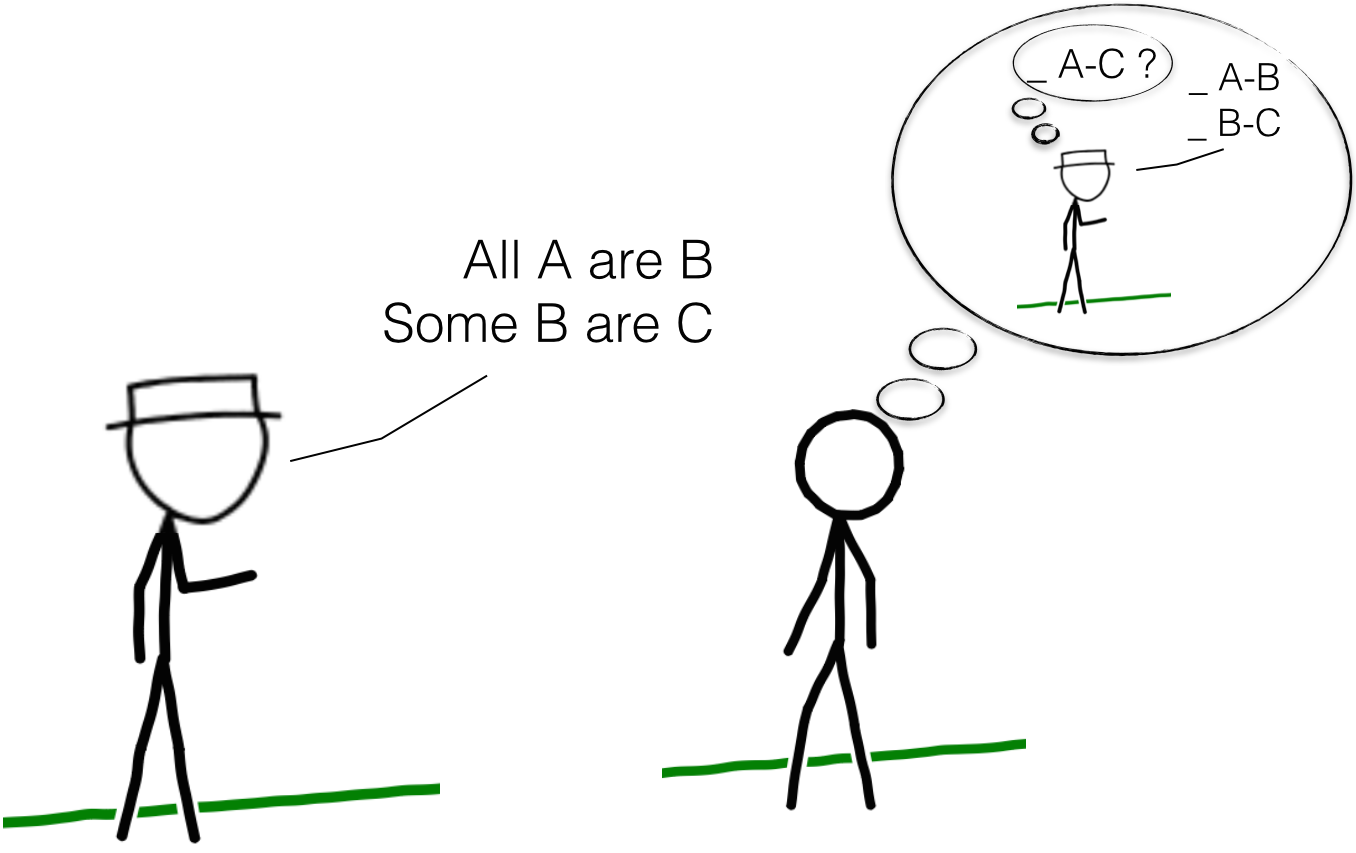
\includegraphics[width=\columnwidth]{fig0_cartoon3}
    \caption{How will the reasoner interpret the experimenter's argument?}
  \label{fig:xkcd}
\end{figure}

Perhaps because of this divergence between human behavior and deductive logic, syllogistic reasoning has been a topic of  interest in cognitive psychology for over a hundred years \cite{storring1908}, and before that in philosophy, dating back to Aristotle. %In cognitive psychology we are interested in how people reason, and syllogisms lie at the intriguing intersection of natural and formal reasoning, of language and logic.%
Syllogisms are undoubtedly logical; indeed, the syllogistic form was the only formal system of logic for millennia. At the same time, the arguments use natural language quantifiers and invite natural language conclusions; precisely pinning down the meaning and use of quantifiers has been an ongoing area of inquiry since Aristotle \cite<e.g.>{negationHorn}.


Many theories of syllogistic reasoning take deduction as a given and try to explain reasoning errors as a matter of noise during cognition. Errors, then, may arise from improper use of deductive rules or biased construction of logical models. 
%In either case, logic makes the connection to natural language semantics natural (though not central).
Many other kinds of reasoning, however, can be well-explained as probabilistic inference under uncertainty. Probability theory provides a natural description of a world in which you don't know exactly how many people are in the hallway outside your door, or whether or not the lion is going to charge.
We suggest that combining probabilistic reasoning with natural language semantics and pragmatics is a useful approach in that knowledge can describe distributions on possible situations, and these distributions can be updated by sentences with new information.
In this formalism, deduction emerges as those arguments which are always true and syllogistic reasoning becomes a process of determining that which is most probable, relevant, and informative.



%
%Theories of syllogistic reasoning have been  One possibility is {\emph{logical deduction}. When a theory takes deduction to be fundamental, the explanatory power of the theory derives from explaining errors in deductive inference. That is to say, these theories treat the variety of performance errors as the first-class explanandum.
%
%We take a different path. We propose, as has been proposed before, that people are reasoning according to their {\emph everyday} mode of reasoning. {\emph Everyday} reasoning is understood as the type of reasoning that is refined for dealing with a world of uncertainty, a world in which you don't know how many people are in the hallway outside your door or whether or not the lion is going to start charging. This type of reasoning is most succinctly described in the language of probability theory. 

\section{A pragmatic Bayesian reasoner model}

Our model begins with the intuition that people reason probabilistically about situations populated by objects with properties. To represent this type of richly structured model, we must go beyond propositional logic and its probabilistic counterpart, Bayesian networks. We instead build our model using the probabilistic programing language Church \cite{Goodman2008}, a kind of higher-order probabilistic logic in which it is natural to describe distributions over objects and their properties. For background and details on this form of model representation, see \url{http://probmods.org}.

Situations are composed of $n$ objects:
\begin{lstlisting}
(define objects (list 'o1 'o2 ... 'on))
\end{lstlisting}
%\lstinline{(define objects (list 'o1 'o2 ...))}. 
(Ellipses indicate omissions for brevity, otherwise models are specified via runnable Church code\footnote{A fully-specified version of this model can be accessed at: \url{http://forestdb.org/models/syllogisms-cogsci14.html}}.)
Properties \lstinline{A}, \lstinline{B}, and \lstinline{C} of these objects are represented as functions from objects to the property value. We assume properties are Boolean, and so property values can be \lstinline{true} or \lstinline{false}. We assume no \emph{a priori} information about the meaning of the properties and thus they are determined independently:
\begin{lstlisting}
(define A (mem (lambda (x) (flip br))))
(define B (mem (lambda (x) (flip br))))
(define C (mem (lambda (x) (flip br))))
\end{lstlisting}
Note that the operator \lstinline{mem} memoizes these functions, so that a given object has the same value each time it is examined within a given situation, even though it is initially determined probabilistically (via \lstinline{flip}). 
%This allows the properties to be defined independently of the set of objects. 
Previous probabilistic models \cite{Oaksford1994} have invoked a principle of rarity from the observation that properties are relatively rare of objects in the world\footnote{This article is an article and it's about reasoning, but it's not a cat, and it's not a car, nor an elephant nor the color red. In fact, there's a very large number of things which this article is not.}. For us, this simply means the base rate, \lstinline{br}, of properties is small.  

%, each with 1, 2 or 3 properties corresponding to the three terms of a syllogism. Situations are sampled from a naive prior. In this setting, it is reasonable to assume that the prior probability, $P(situation)$, is a binomial distribution (i.e. the probability of a coin of a given weight coming up Heads $n$ times in a row, where $n$ is the number of objects). We assume properties are relatively rare of objects; this means the base rate (\lstinline{br}) of properties is less than 0.50.  This principle of rarity comes from the intuition that properties are relative rare \footnote{This article is an article and it's about reasoning, but it's not a cat, and it's not a car, nor an elephant nor the color red. In fact, there's a very large number of things which this article is not.}, and this has been used in probabilistic models previously. 
%
%\begin{lstlisting}
%(define A (mem (lambda (x) (flip br))))
%(define B (mem (lambda (x) (flip br))))
%(define C (mem (lambda (x) (flip br))))
%\end{lstlisting}



%The motivation for our model stems from the intuitions that people reason by constructing situations consistent with their probabilistic prior knowledge, and they interpret premises and choosing conclusions as 
%
%



We interpret quantifiers as truth-functional operators, consistent with standard practice in formal semantics.
A quantifier (e.g. \lstinline{all}) is a function of two properties (e.g. \lstinline{A} and \lstinline{B}) which maps to a truth value by consulting the properties of the objects in the current situation. For instance:
\begin{lstlisting}
(define all 
  (lambda (A B) 
    (all-true (map (lambda (x) (if (A x) (B x) true)) 
                   objects))))
\end{lstlisting}
Here the helper function \lstinline{all-true} simply checks that all elements of a list are true, i.e. that all the \emph{As} are indeed \emph{Bs}. The function \lstinline{map} applies the given function ---\lstinline{(lambda ...)}--- to each element of the list \lstinline{objects}. Similarly we can define \lstinline{some}, \lstinline{none}, \lstinline{not-all} to have their standard meanings. For a first test of the model, we assume sets are non-empty, i.e. \lstinline{all} and \lstinline{none} cannot be trivially true.

The key observation to connect these truth-functional meanings of quantifier expressions to probability distributions over situations is that an expression which assigns a Boolean value to each situation can be used for probabilistic conditioning. That is, these quantifier expressions can be used to update a prior belief distribution over situations into a posterior belief distribution. For syllogistic reasoning we are interested not in the posterior distribution over situations \emph{per se}, but the distribution on true conclusions that these situations imply. In Church this looks like:
\begin{lstlisting}
(query
 (define objects (list 'o1 'o2 ... 'on))
 . . . define A,B,C . . .
 . . . define all, some, no, not-all . . .
 (define conclusion (conclusion-prior))
 
 conclusion
 
 (and (conclusion A C) 
      (premise-one A B)
      (premise-two B C)))
\end{lstlisting}

The first arguments to a query function are a generative model: definitions or the background knowledge with which a reasoning agent is endowed. Definitions for which a prior is stipulated (e.g. \lstinline{conclusion}) denote aspects of the world over which the agent has uncertainty. The second argument, called the \emph{query expression}, is the aspect of the computation about which we are interested; it is what we want to know. The final argument, called the \emph{conditioner}, is the information with which we update our beliefs; it is what we know. We assume that the prior distribution over conclusions (and premises, below) is uniform.

%The Conditional Semantics model treats the premises of a syllogism as evidence by which to update its belief prior over propositions (which are now potential conclusions). This update rule we take to be probabilistic conditioning. Thus, we get a posterior distribution of propositions, conditioned on premises being true. This has the nice feature of returning a degree of belief in each of the possible conclusions for every syllogism. Using this, we can test the hypothesis that reasoners in syllogistic reasoning tasks are essentially drawing samples from the posterior distribution of the conclusion conditioned on the premises (so-called ``posterior matching") \cite{Griffiths2006}.
%
%\begin{lstlisting}
%(query
%  ...define A,B,C...
%  (define conclusion (conclusion-prior))
%  
%  conclusion
%  
%  (and (conclusion A C)
%  	 (premise-one A B)
%     (premise-two B C))
%\end{lstlisting}


\subsection{Recursion and pragmatics}
%One reason to be skeptical of mere \emph{posterior matching} in syllogistic reasoning is that language understanding and language production are central to the syllogistic task, and truth-functional semantics can only go so far. 
We have suggested viewing syllogistic reasoning as a case of communication, and this in turn suggests that reasoning should go beyond the semantics of language, to its pragmatics.
%Natural language pragmatics could enter in two places in the above model: premise interpretation and conclusion production. %
%We address premise interpretation in this paper.%


Following the \emph{rational speech-act} (RSA) theory \cite{Goodman2013,Frank2012a}, we imagine a reasoner who receives premises from an informative speaker. The speaker conveys information about which only she has access -- in RSA, her access was a current state of the world. By being informative with respect to the world-state, the speaker is able to communicate enriched meanings (e.g. scalar implicature -- that ``some" may also imply ``not all"). It is known, however, that standalone scalar implicatures do a poor job of accounting for reasoning with syllogisms \cite{Roberts2001}. Indeed, a preliminary analysis of a standard Gricean-listener model in this framework was consistent with this account. 

However, a listener (our reasoner) may consider the premises in a wider, conversational setting: she may ask herself why the experimenter chose to give these particular premises, as opposed to alternative arguments. This requires a closer look at what the reasoner believes to be at issue in this ``conversation''---the Question Under Discussion, or QUD \cite{Roberts2004QUD}. In a syllogistic context, we take the QUD to be ``what is the relationship between A \& C (the end terms)?", very often the actual context in which the experiment is presented. 

In this setup, pragmatic inferences will differ from the standard local implicatures; for instance, ``Some A are B'' may not lead to a ``Not all A are B'' implicature if ``All A are B'' wouldn't provide additional information about the A-C relationship. The enriched meanings come from the following counter-factual consideration: ``why did this experimenter present me with this argument and not any other argument?" The pragmatic reasoner enriches the conclusions that are more uniquely determined by the particular argument the experimenter provides.

The A-C QUD is naturally captured by a \lstinline{reasoner} who considers an \lstinline{experimenter} who considers the conclusions the \lstinline{reasoner} would draw about A \& C (not the reasoner's inferences about the whole world-state, which would---superfluously---include B).

%Following the Rational Speech Act theory \cite{Goodman2013,Frank2012a} we imagine a reasoner who chooses the conclusions which are more likely to convey information about which only the reasoner has access---in this case, the premises. That is, we imagine that the reasoner treats the conclusion as a message chosen for a listener who lacks the premises (or perhaps lacks only the ability to reason from premises to conclusions).
%This listener can be thought of concretely as the (rather naive) person evaluating the participant's responses. In the original Rational Speech Act model, the listener hears an utterance and tries to reconstruct the situation observed by the speaker. In our model, the \emph{conclusion-listener} hears a conclusion and tries to reconstruct the premises with which the reasoner was presented. This distinction between situation and premise reconstruction turns out to be important as the reasoner does not observe a situation directly but rather only constructs situations consistent with the premises: our reasoner attempts to convey her \emph{knowledge state}, not her guess about the situation.


%In the model, the \lstinline{reasoner} considers an agent who is selecting premises according to the conclusion the literal \emph{reasoner} is likely to draw. The agent who receives the conclusion from the \lstinline{reasoner} described above and the agent that provides the premises are each tasked with selecting premises based on a conclusion as input. The only difference is that the agent that provides the premises is grounded in the truth of the premises while the agent that receives the conclusion is grounded in the conclusion being true. Because of this, we can formalize the two into a single function -- the \lstinline{questioner}.

We can combine the above intuitions about pragmatic comprehension into a model in which \lstinline{reasoner} and \lstinline{experimenter} jointly reason about each other. Critically, each agent reasons about the other at recursive \lstinline{depth} of comprehension:
\begin{lstlisting}
(define (experimenter conclusion depth)
  (query 
   (define premises (premise-prior))
   
   premises
   
   (equal? conclusion (softmax (reasoner premises depth) alpha))))

(define (reasoner premises depth)
  (query 
   (define objects (list 'o1 'o2 ... 'on)) 
   . . . define A,B,C . . . 
   . . . define all, some, no, not-all . . .
   (define conclusion (conclusion-prior))
   
   conclusion
   
   (and (conclusion A C)
	   (if (depth 0)
          (and ((first premises) A B)
               ((second premises) B C))
          (equal? premises (experimenter conclusion (- depth 1)))))))
            
\end{lstlisting}


The \lstinline{reasoner} and \lstinline{experimenter} functions produce a distribution over conclusions and premises\footnote{As a first pass, we consider the alternative premises generated by \lstinline{premise-prior} to be the set of all premises of the same term orderings, i.e. alternative quantifiers, keeping the structure of the sentences fixed.}, respectively. Since we take these functions to represent actual persons in a communicative setting, we take premises to be selected from these distributions according to a Luce choice, or \lstinline{softmax}, decision rule with a parameter \lstinline{alpha} that denotes the degree to which argument is chosen optimally \cite{luce1959}. This takes the distribution, raises it to a power \lstinline{alpha} and renormalizes. As \lstinline{depth} increases, the premises becomes more informative with respect to the uniquely-implicated conclusions (unique, that is, for those premises). When \lstinline{depth} is 0, the model collapses to produce the $P$(conclusion $\arrowvert$ premises), which we refer to as the \emph{literal Bayesian reasoner}. We refer to the model with \lstinline{depth} equal\footnote{To a first approximation, increasing \lstinline{depth} to greater than 1 produces results  similar to increasing \lstinline{alpha}.} to 1 as the \emph{pragmatic Bayesian reasoner}. 
%Using this framework, we can investigate the complementary influences of pragmatic interpretation of premises and production of conclusions. %

The three parameters of the model---\lstinline{n_objects}, \lstinline{br}, and \lstinline{alpha}---were fit by maximum-likelihood estimation. These fit parameter values were 5, 0.25, and 4.75, respectively.%\footnote{n.b. \lstinline{n_objects} = 5 keeps the number of distinct objects in a situation to a minimum while \lstinline{br} = 0.25 is in accord with the rarity assumption.}%.


%addresses the problem of language understanding as that of a speaker trying to convey information about a world or situation that the speaker has observed \cite{Goodman2013,Frank2012a}. The speaker draws on common-ground of communicative goals to maximize information content of a given utterance. In particular, choosing an utterance in proportion to the likelihood of a listener inferring the situations about which the speaker wishes to convey information. In turn, a listener considers situations in which the given utterance heard is not only true but would be chosen to disambiguate amongst multiple consistent situations by an informatve speaker. This results in the canonical ``scalar implicature" wherein the literal meaning of ``{\em some} of the apples are red" is enriched to communicate ``some {\em but not all} of the apples are red".
%
%We use a variant of the nested-conditioning model of scalar implicature \cite{Goodman2013} to break the symmetry described above. We treat the reasoner as a sort of pragmatic speaker with a hypothetical listener in the reasoner's mental representation. This listener can be thought of concretely as the person evaluating the participant's responses. In the original scalar implicature model, the listener hears an utterance and tries to reconstruct the situation observed by the speaker. In our model, the listener hears the conclusion and tries to reconstruct the premises with which the reasoner was presented. This distinction turns out to be important as the reasoner does not observe a situation directly but rather constructs situations consistent with the premises. 
%
%
%
%
%To illustrate pragmatic production, we offer as an example the canonical ``All/all" syllogism:
%
%\begin{quotation}
%All As are Bs \\
%All Bs are Cs \\
%\end{quotation}
%
%This is in fact one of the easiest syllogisms to which 81\% of participants produce the valid{\emph All As are Cs} conclusion. The other valid conclusions -- \emph{Some As are Cs} and \emph{Some Cs are As} receive only 7\% of the endorsements. However, in every possible situation in which {\emph All As are Cs} is true, \emph{Some As are Cs} and \emph{Some Cs are As} are also true. That is, they are equally probable given the posterior. 
%
%This illustrates one of the issues with the conditional semantics model: it is too literal. The model computes the probability of the conclusion conditioned on the premises being true. For logically valid syllogistic conclusion, this probability is equal to 1. In particular, for any syllogism for which one of the universal quantifiers is valid (i.e. {\emph all} and {\emph none}), the particular quantifier (i.e.{\emph some} and {\emph not all}, respectively) will also be valid. Human reasoners show a clear preference for conclusions using universal quantifiers (all and none) in these cases. 
%
%
%
%
%Preliminary analyses suggest that standard Gricean implicatures (for instance ``some'' implies ``not all'') have a minimal additional effect on model predictions. This is consistent with other empirical findings which set out to test this question directly \cite{??}. 
%However we speculate that other important pragmatic effects may be important for the interpretation of the premises: existential presupposition and relevance of the middle term.
%%
%For the current initial exploration we evaluate these effects by building them into the prior distribution and literal semantics for simplicity \red{(which is lame)}.
%%
%Existential presupposition, a notion which goes back to Aristotle, is simply the observation that it is inconsistent to say ``All A are B'' if there are no objects with property A (and similarly for other quantifiers). \red{check with model..} We can simply add this to the literal meaning (the definition) of each quantifier. \red{cf pragmatic alternative ``No As''.}
%
%A second potential interpretation effect comes from the following question: In what natural setting would a reasonable person produce a syllogistic  argument? 
%Why would anyone ever go through the hassle of uttering two sentences which do not convey the totality of what is intended to be conveyed? 
%We suggest this is often due to an asymmetry among the three relations (i.e. A-B, B-C, C-A): A is more directly related to B that to C, etc.
%If this is the situation under which someone would bother to utter syllogistic premises, then the reasoner should assume this to be the the case in reasoning about the syllogism.
%%We posit that the A-B \& B-C relations are weighted more strongly than the A-C relationship, possibly owing to common ground of those relationships. In some way, A-C is unexpected, or somewhat unbelievable. If it weren't, there would be no reason to work through the syllogism. 
%%The syllogism was invented as a tool of argument, to convince others. Nobody needs convincing that ``Socrates is mortal". 
%We capture this intuition, by introducing dependence into the prior between A \& B, and B \& C:
%% a small dependency into the prior such that A \& C are more likely when B is present and less likely when B is absent. 
% \begin{lstlisting}
%(define B (mem (lambda (x) (flip br))))
%(define A (mem (lambda (x) 
%                 (flip (if (B x) (+ br df) (- br df))))))
%(define C (mem (lambda (x) 
%                 (flip (if (B x) (+ br df) (- br df))))))
%\end{lstlisting}
%In our example from the beginning, this means that a person being out of the office for weeks is less likely if they don't have the flu and more likely if they do have the flu. 


\section{Results}

%\subsection{Meta-analysis data}
To test the predictions of the model we used data from the meta-analysis of syllogistic reasoning tasks presented by \citeA{Chater1999}. These data were compiled from five studies on syllogistic reasoning, completed from 1978-1984. The data include percentage response for conclusions that contain each of the 4 quantifiers as well as for ``No Valid Conclusion" (NVC). The Bayesian reasoning models described so far are not equipped to handle NVC\footnote{In each possible situation, at least one of the four conclusions will be true. In fact, since the four possible quantifiers form two pairs of logical contradictions, exactly two conclusions will be true in each situation.  For example, \emph{all} and \emph{not all} cannot both be true, but one must be true. The same is the case for \emph{none} and \emph{some}.}. We removed the NVC responses from the meta-analysis and renormalized so the endorsement of all conclusions for a syllogism adds to 100. Some studies in the meta-analysis asked participants to draw conclusions which were restricted to the classical ordering of terms (C-A) while others allowed conclusions in either direction (A-C or C-A). To accommodate this, we allowed our model to draw conclusions in either order and collapsed responses across these two orderings to compare it to this data set.
\subsection{Qualitative results}For each model, we report the total number of syllogisms for which the model's modal response is the same as for in the meta-analysis data. This is a qualitative assessment of fit. The table below shows the number of modal responses for which the model matched the data (columns ``matches"). We separate these into valid and invalid syllogisms\footnote{Since the response format in the meta-analysis varied across studies, the number of valid syllogisms was also not the same. Here we count as valid only the syllogisms that would have been considered valid in all studies.}. The total numbers of valid and invalid syllogisms are 24 and 40, respectively. 
\begin{tabular}{l*{3}{c}r}
Model              & matches$_{valid}$ & matches$_{invalid}$ & r$_{valid}$ & r$_{invalid}$  \\
\hline
Prior & 5 & 24 & -.46 & .41  \\
Literal & 17 & 20 & -.20 & .64  \\
Pragmatic & 17 & 26 & .77 & .74 \\
\end{tabular}

As a baseline, we first examined the posterior distribution of conclusions conditioned only on the truth of the conclusion (what we refer to as the ``Prior") to see if it alone accounted for human reasoning patterns. It did not (Figure \ref{fig:megaScatter}, column 1). Since \emph{not all X are Y} is the most likely conclusion to be true, the Prior matches only the syllogisms with a \emph{not all} modal response. 
%
The literal Bayesian reasoner matches the modal response on 37 of the 64 syllogisms. The 29 syllogisms for which \emph{not all} was the modal response are qualitatively unaffected. The model also matches 8 syllogisms for which \emph{some} and \emph{none} are favored (e.g., Figure \ref{fig:barplots}, [2]). Probabilistic reasoning introduces gradation to inference which accounts for an appreciable portion of the variance.
%
\begin{figure}
\centering
    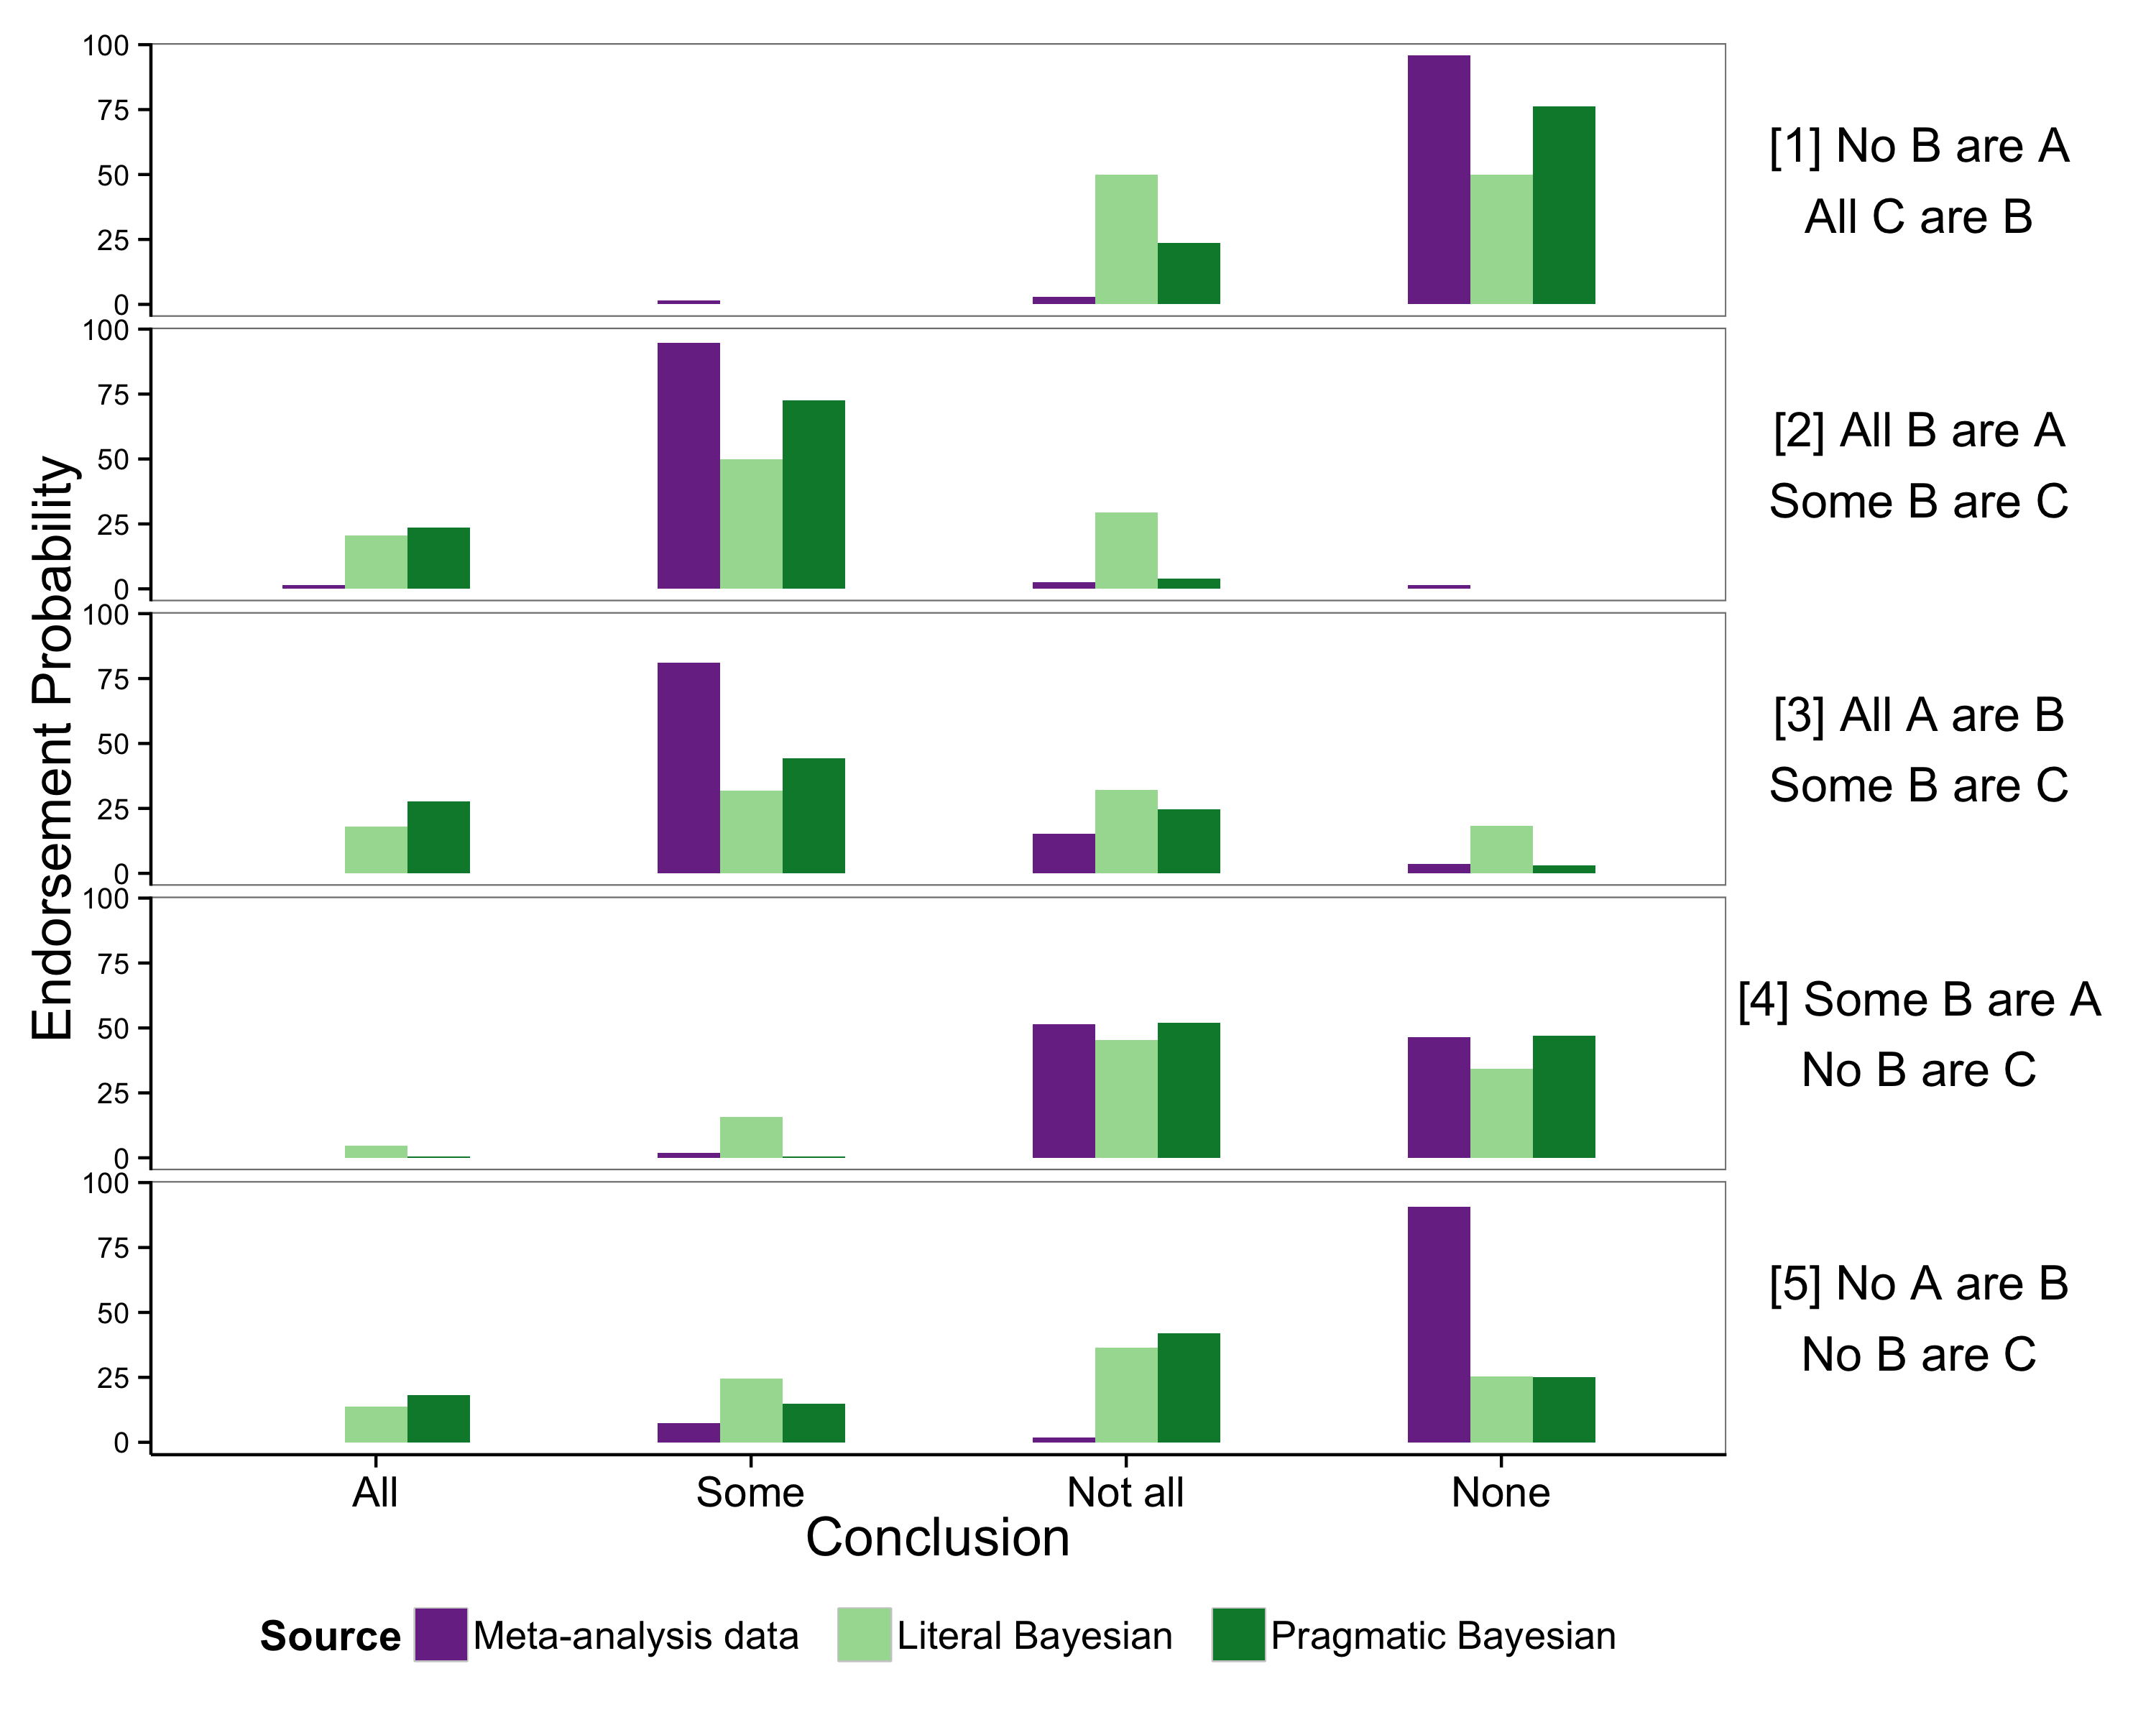
\includegraphics[width=\columnwidth]{multibar_fig1}
    \caption{Five example syllogisms. 
    [1] Literal reasoner  has no preference among equally valid conclusions; the symmetry is broken by the pragmatic reasoner who considers the argument in the space of possible arguments.     
    [2] Literal reasoner alone captures the modal response and pragmatics enriches the quantitative fit.     
    [3] Relatively informative premises suggest \emph{some} is the most likely interpretation. 
    [4] Models are able to capture multiple preferred conclusions. 
    [5] Models do poorly in matching subjects' responses in an uninformative, invalid syllogism.}
  \label{fig:barplots}
\end{figure}

%Introducing pragmatics into the model, we consider first production---PQR$_{0,1}$. The model now distinguishes between equally valid conclusions on the basis of informativity (e.g. Figure \ref{fig:barplots} [1], column 4). The model selects not only conclusions likely to be true, but also informative, and now matches 42 out of 64 modal responses. %
%


Conversational pragmatics can enrich the meaning of the premises given to the pragmatic reasoner by considering ``why has the experimenter produced this argument --- these premises --- given that she may have given other arguments?'' 
%Critically, the reasoner does not consider these alternatives with respect to the full state of the world (i.e. the sets A, B and C) but rather only with respect to the QUD (i.e. the sets A and C, marginalizing out B). This captures the intuition that people are considering specifically the relationship between A \& C.
The pragmatic Bayesian maximally-prefers the modal response of subjects for 43 out of 64 syllogisms. As well, it picks up on some of the subtle phenomena present in syllogistic reasoning. Example [3] in Figure \ref{fig:barplots} is one such case. The premises considered literally are relatively uninformative. The literal reasoner is very similar to the Prior (not shown in Figure \ref{fig:barplots}; but see Figure \ref{fig:megaScatter}, column 1). Many arguments in the syllogistic space, however, do not update the prior substantially. As such, the most probable conclusion given all arguments is  \emph{not all X are Y}. Since the argument in [3] is more informative relative to others (e.g. the argument in [5]), the most likely intention of the imagined experimenter was to convey that \emph{some A are C}.

In addition to capturing many of the modal responses, the model is able to accommodate more than one plausible conclusion. Example [4] in Figure \ref{fig:barplots} is one such example. This is a syllogism with a valid conclusion, but one which people find difficult to draw. The literal reasoner model tells us why: in many of the possible situations in which the premises are true, a \emph{none} conclusion is true. In addition, \emph{none} is a difficult conclusion to convey in an argument---relative to \emph{not all}---and so the pragmatic Bayesian strengthens the plausible but invalid \emph{none}.

Though this is encouraging qualitative data, there are a number of syllogisms for which reasoning patterns are not accounted for by the pragmatic Bayesian reasoner. Many of these are syllogisms use two negative quantifiers (\emph{not all} or \emph{none}) as the premises. For these arguments, the predictions of the literal reasoner do not differ appreciably from the predictions of the Prior (Figure \ref{fig:barplots}, [5]), because the rarity prior assumes most relations will be false to begin with. 

\subsection{Model fit}

To assess our models' quantitative fits we examine correlations across all 256 data points (64 syllogisms x 4 conclusions), shown in Figure \ref{fig:megaScatter}.
%
The Prior's predictions are the same for all syllogisms and the overall fit is poor (r = 0.36).  After conditioning on the truth of the premises, the model is able to make graded responses. These responses are a reflection of the types of situations consistent with the premises. The overall correlation is appreciably higher (r = 0.64). Among valid conclusions, however, (squares in Figure \ref{fig:megaScatter}) the fit is terrible (r = -0.20 for valid conclusions only). This is a direct consequence of the reasoner's literalness: the model has no preference among multiple valid conclusions, since a valid conclusion -- by definition -- is one which is true in every situation in which the premises are true\footnote{An upper bound of 50 percent endorsement emerges from the fact that the 4 quantifiers form 2 sets of logical contradictions. Each pair of quantifiers has something true in each situation; thus, the maximum endorsement after normalization is 50.}.

This symmetry is broken by the reasoner who interprets the premises as coming from a pragmatic experimenter (Figure \ref{fig:megaScatter}, column 3), and the overall fit improves (r = 0.77). The model is now able to make graded responses among valid conclusions (r = 0.77 for valid conclusions only). 



%The reasoner who takes the premises at face value but who produces conclusions to be informative---PQR$_{0,1}$---has also a better fit than the literal model (r = 0.69) and the fit among valid conclusions is even stronger (r = 0.82 for valid conclusions only). %

%PQR$_{1,1}$---which reasons pragmatically on both the production and the interpretation---does not model the data overall any better than the individual processes. This joint model selects the modal response on 41 out of the 64 syllogisms and provides a worse fit than either of the individual PQR models (r = 0.66). However, among valid conclusions the correlation is highest (r = 0.85). This mismatch is puzzling and likely due to the particular way in which the information between the two inference processes is shared.  We leave for later work the proper way of combining information from the two loci of pragmatic inference.%


%We compared these results to those found when using a uniform prior (\ref{fig:megaScatter}, row 1)) and found the overall fit much better with the binomial, which invokes the principle of rarity. 

\begin{figure*}[t!] %[htp]
\centering
	\subfigure
		\centering
  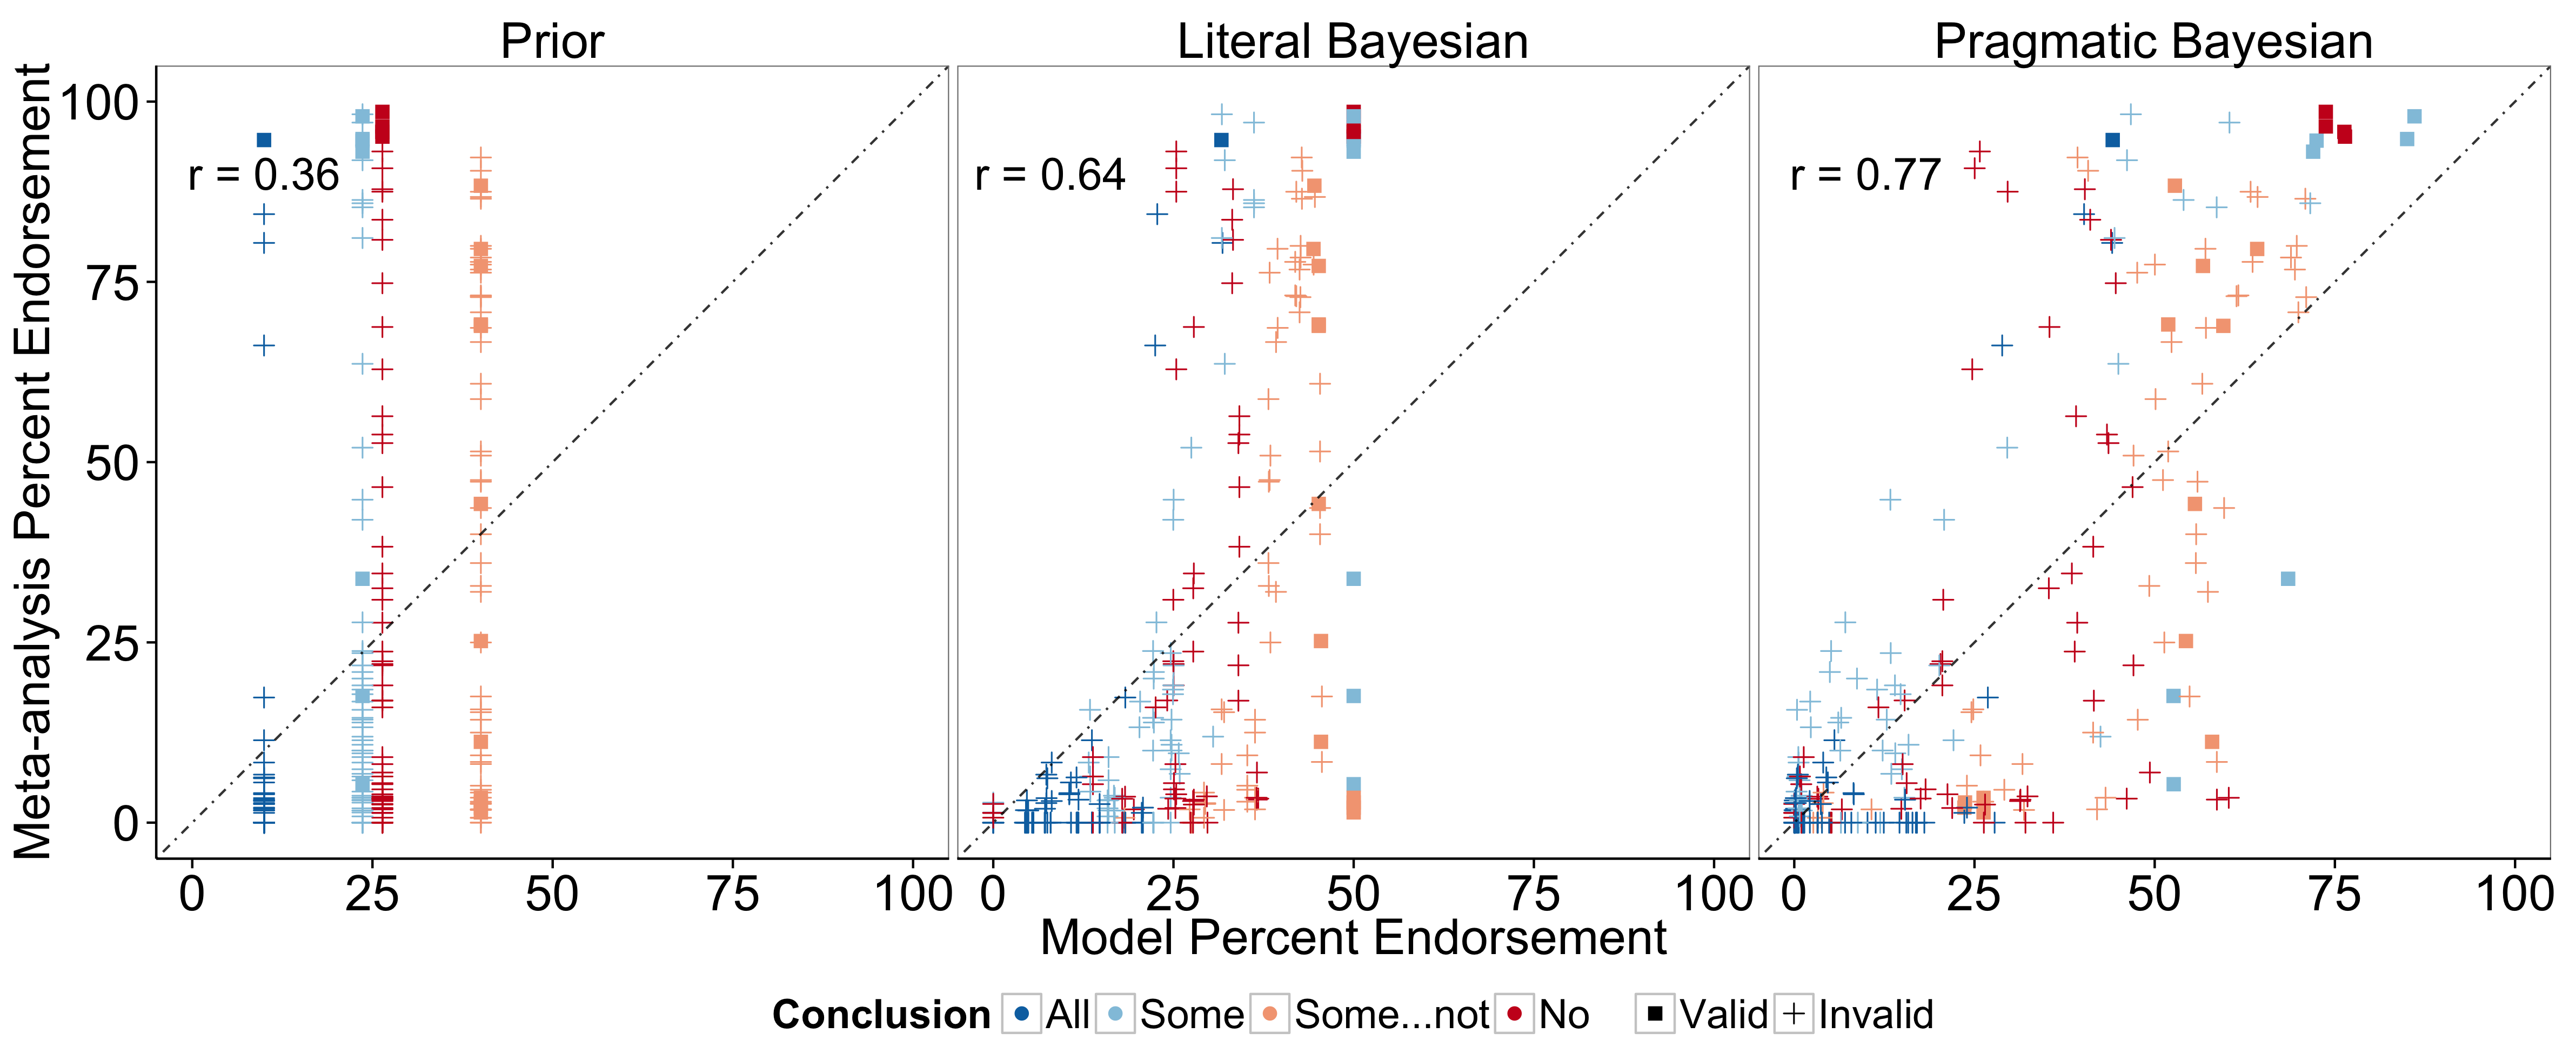
\includegraphics[width=\textwidth]{multiScatter_fig2}
  \caption{Human subject percentage endorsement vs. model predictions.
  Columns (from L to R): predictions based only on the prior---$P($conclusion$)$; literal Bayesian reasoner---$P($conclusion $\arrowvert$ premises$)$; and the pragmatic Bayesian reasoner (see text).}
  \label{fig:megaScatter}

\end{figure*}

%\subsection{Dependency}



%Using the correlated prior, the Conditional Semantics model gets 45 out of 64 modal responses. The overall fit is also improved, r = 0.75 (Figure \ref{fig:megaScatter}, row 3). The Conditional Pragmatics model does better as well, predicted the modal response for 52 syllogisms. Additionally, the quantitative fit is high (r = 0.85). Among valid syllogisms, it is correspondingly higher as well (r = 0.88). 


\section{Generalized quantifiers}

Our model is based on a truth-functional semantics and as such, it is able to accommodate any quantified sentence with a truth-functional meaning. The meaning of generalized quantifiers like ``most" and ``few" is a topic of debate in formal semantics, but can be modeled to a first approximation as a thresholded function. As a first test of the generality of the model, we define most and few by a threshold of 0.5 such that ``most As are Bs" is true if more than half of the As are Bs. Once we have added these lexical items, the Bayesian reasoning models extend naturally. 
%
We compare our model predictions to two studies carried out by \citeA{Chater1999} on syllogisms using the generalized quantifiers \emph{most} and \emph{few} e.g. \emph{Most artists are beekeepers; Few chemists are beekeepers}. Participants were told to indicate which, if any, of the four quantifier conclusions followed from the premises and were allowed to select multiple options.
%
The set of syllogisms was divided into two experiments to avoid subject fatigue.

\begin{figure*}[t]
	\centering
  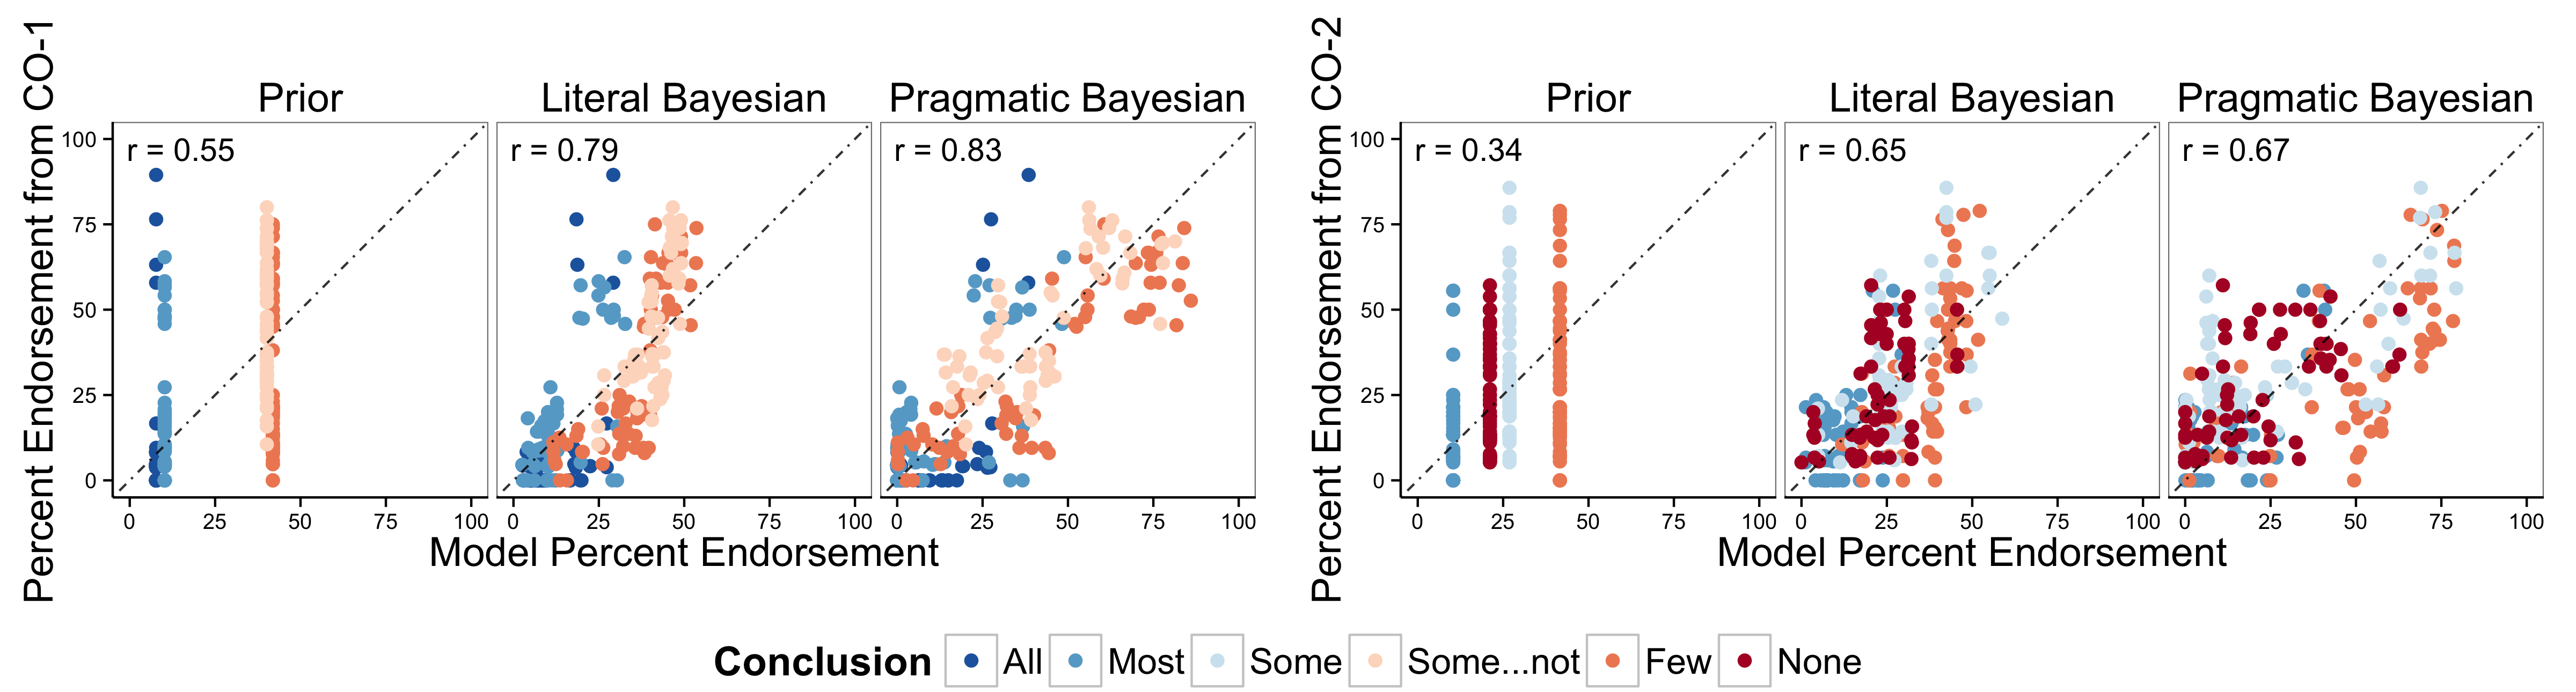
\includegraphics[width=\textwidth]{fig4_multiScatter_colorset_AMFO_MFIE_n6_br0,30}
      \caption{Human subject percentage endorsement vs. model fits for 2 experiments using generalized quantifiers. Experiment 1 (left) used the quantifiers \{\emph{all}, \emph{most}, \emph{few}, \emph{not all}\}. Experiment 2 (right) used the quantifiers \{\emph{most}, \emph{few}, \emph{some}, \emph{none}\}.}
  \label{fig:mfScatter}
\end{figure*}


We find good correspondence between the experimental data and the model, even with only a local parameter search\footnote{ \lstinline{n_objects} fit to 6, \lstinline{br} to 0.30, \lstinline{alpha} to 4.75. The words ``most" and ``few" might pragmatically implicate sets of substantially larger size, and thus the data might be captured better by searching over a larger parameter space for  \lstinline{n_objects}.  In this analysis, we examined only a small search radius around the parameter estimates used to model the meta-analysis data.} (Figure \ref{fig:mfScatter}). In Experiment 1, the quantifiers \emph{all}, \emph{most}, \emph{few}, and \emph{not all} were used. In Experiment 2, the quantifiers \emph{most}, \emph{few}, \emph{some}, and \emph{none} were used. Note again the total number of syllogisms in an experiment is 64.
\begin{tabular}{l*{3}{c}r}
Model              & matches$_{Exp_{1}}$ & matches$_{Exp_{2}}$ & r$_{Exp_{1}}$ & r$_{Exp_{2}}$  \\
\hline
Prior & 23 & 23 & .55 & .34  \\
Literal & 42 & 36 & .79 & .65   \\
Pragmatic & 47 & 35 & .83 & .67  \\
\end{tabular}

%The PQR$_{0,0}$ model selected the modal response for 45 out of 64 syllogisms and had a good quantitative fit (r = 0.79).  PQR$_{1,0}$ selected 48 modal responses and had an even better quantitative fit (r = 0.81). PQR$_{0,1}$ selected 50 modal responses and had a slightly worse fit (r = 0.76). 
%

%PQR$_{0,0}$ selected the modal response for 34 out of 64 syllogisms and had a correlation of r = 0.63. PQR$_{1,0}$ selected 43 modal responses with  r = 0.63. PQR$_{0,1}$ selected 44 modal responses and had a slightly worse fit r = 0.60. 
%
The fit is appreciably better for Experiment 1 than for Experiment 2, and the same was true for the Probability Heuristics Model (r = 0.94 vs r = 0.63). Overall, the proportion of \emph{no valid conclusion} responses in the experimental data, which we do not model, was much higher in Experiment 2 than in Experiment 1. This may explain why the pragmatic reasoner tends to give high endorsement to many conclusions which people do not (Figure \ref{fig:mfScatter}, rightmost scatterplot). A model that takes into account NVC may alleviate this effect.


\section{Discussion}

The inspiration for the pragmatic Bayesian reasoning model comes from the idea that syllogistic reasoning cannot be disentangled from language understanding. Natural language semantics alone seems to be insufficient to explain the variability in reasoning, however. We have shown that a combination of semantics and conversational pragmatics provides insight into how people reason with syllogistic arguments. 

A recent meta-analysis carved the space of reasoning theories into three partitions: those based on models or diagrammatic reasoning, those based on formal logical rules, and those based on heuristics \cite{Khemlani2012}. We see the space slightly differently. In one dimension, theories are based on the direct application of derivation rules---be they heuristic or logical---or they are based on the construction of concrete representations or models. In another dimension, theories may fundamentally be interested in deductive validity or probabilistic support. This theoretical partitioning places the Bayesian reasoning models presented here in a previously unexplored quadrant of the two-dimensional theoretical space described: we consider probabilistic reasoning over concrete situations.

Mental Models Theory (MMT) was offered to capture the intuition that people are able to reason about sets of things explicitly and with respect to context by constructing mental representations of individuals over which to reason. The situations described in our computational models are analogous to mental models. To address the problem of determining which models come into existence, however, MMT relies on a number of complex heuristics. By contrast, we derive a distribution over models (or situations) from natural language semantics and pragmatics, with no further assumptions.

%In LBR the situations follow from the semantic assumptions and fundamental laws of probability with no further assumptions; pragmatics then modifies this well-defined reasoning process.%

\citeA{Chater1999} introduced the Probability Heuristic Model (PHM) which derives a set of probabilistic rules for syllogistic reasoning; to account for informativity and other effects, the PHM then augments these probabilistic rules with a complex set of heuristics (for example, informative-conclusion heuristics). Our model differs in two respects. First, the probabilistic ``rules'' emerge from the semantics of quantifiers by reasoning about situations. Second, we strengthen inferences by employing previously-proposed formalisms for pragmatic reasoning. This gives rise to many of the same effects, such as informativity, without postulating heuristics \emph{de novo}.

%from the intuition that people are using \emph{everyday} reasoning when asked to resolve syllogisms. To accomplish this, the PHM uses a number of heuristics and derives an ordering of informativity for the various quantifiers. PQR also has an ordering of informativity. The difference is that PHM's ordering is derived at the propositional level, using a probabilistic semantics, by assuming categories are represented as hyperspheres in a high-dimensional concept space. PQR uses a truth-functional semantics which it applies to samples from a distribution over situations. An ordering of informativity emerges from the fact that not all quantified propositions are equally likely across situations.

%Additionally, very nature of the heuristics on which the PHM relies to produce and quantify confidence in conclusions suggests reasoners are engaging with syllogisms at a propositional level and not at the level of concrete representations. In this way, we consider heuristic accounts analogous to formal rule theories (e.g. \citeA{rips1994}) in that people are reasoning at the level of propositions, albeit probabilistic propositions. PQR is different in that it operates at the level of concrete representations.

The syllogistic reasoning task involves reading a pair of sentences and producing or evaluating a conclusion. We have considered the pragmatics of argument interpretation---the problem the reasoner faces when given some sentences. Natural language pragmatics may also enter into the production of a conclusion (for tasks that require production). The reasoner is likely tempted to produce conclusions which are not only true but also good, or \emph{informative}. At the same time, the option of ``no valid conclusion"---of saying nothing---looms large for the reasoner. We leave for future work the incorporation of production of informative conclusions as well as the ability to say ``nothing follows".


%Natural language pragmatics could enter in two places in the above model: premise interpretation and conclusion production. %
%We address premise interpretation in this paper.%

%The pragmatic Bayesian reasoner accounts for much of the data. The number of syllogisms whose modal response was not predicted by either model is a mere 9 (i.e. 55 out of 64 syllogisms were accounted for by one of the models). However, PQR$_{1,1}$ in its current formulation is not simply a sum of its parts. Evidence from the individual models suggests some complex interaction between pragmatic interpretation of premises and production of conclusions is at work in human reasoning behavior. %


\section{Conclusion}

This is early work and we have found promising evidence, both qualitative and quantitative, that this framework will allow for a more explicit understanding of syllogistic reasoning. 
%PQR$_{1,0}$ explores pragmatic interpretation of premises. It does so not with the goal of inferring the true situation but only the question-under-discussion. Thus, PQR captures an aspect of the reasoning data wherein pragmatic interpretation extends beyond standard Gricean implicatures.


A major virtue of the pragmatic reasoning framework is that it extends naturally to incorporate any terms for which a truth-functional semantics can be given.
For instance, we tested the model on \emph{most} and \emph{few} using the simplest, most standard semantics (most is more than half, etc). It is likely that these quantifiers actually have more complex semantics, but even so we accounted for a significant fraction of the data.

In this framework, a syllogism is read as an argument given as a part of discourse between interlocutors. Indeed, this is how syllogisms were used in the time of Aristotle and in the long tradition of scholastic philosophers since. Fundamentally, syllogisms are a tool used to convince others. The results of the pragmatic Bayesian reasoner recast the ancient idea that human reasoning behavior is as much reason as it is human. Gauging degrees of truth or plausibility alone is not sufficient. An agent needs to be posited at the other end of the line so that a conclusion makes sense; so that an argument may convince!

\bibliographystyle{apacite}

\setlength{\bibleftmargin}{.125in}
\setlength{\bibindent}{-\bibleftmargin}

\bibliography{mhtbib}


\end{document}

%If one accepts that the purpose of a syllogism is to convince, a natural question arises. Why not just assert ``Some of my colleagues won't be at work for weeks" from the get-go? Why go through the trouble of laying out premises and having a person draw the conclusion? Arguments are used to persuade, and not all assertions are equally believable \emph{a priori}. The reason premises are presented in this way is that there is no reason to believe some  colleagues will be out of work for weeks. That only happens around Christmas. And so the conclusion is not obvious, and the premises are an alternative route to persuasion. If we accept the premises, we are left with no choice but to draw the conclusion.




























%
%
%We have presented a formal model of syllogistic reasoning based on the \emph{Rational Speech-act} framework. This formalizes the notion that reasoners construct mental situations by sampling and reasoning over these situations, much like has been described in the Mental Models literature. Unlike Mental Models, however, PQR is inherently probabilistic and thus assumes reasoners are in some way gaging degrees of plausibility in syllogistic reasoning tasks. Further, PQR is fundamentally quantitative, and thus can be considered an elaboration of the Mental Models theory.
%
%
%
%\section{Relationship to previous theories}
%
%
%We now review 2 theories which we take to exemplify two of the four quadrants of this theoretical space. 
%
%\subsection{Mental Models}
% The Mental Models Theory (MMT) describes a psychological process by which people reason by constructing {\em iconic} mental representations or models, which represent the terms of a proposition as a collection of individuals. In syllogistic reasoning, a model is constructed for each premise, and premise models are consolidated so that the conclusion may be ``read off" the joint model. For example, a model for the premise  \emph{All colleagues have the flu} could be represented as the following situation.
%
%\begin{tabular}{l l}
%colleague & flu\\
%colleague & flu\\
% & flu\\
%\end{tabular}
%
%This shows 2 individuals who are colleagues and have the flu, and one individual who is not a colleague and has the flu. Thus, each row is a representation of the properties of an individual. MMT emphasizes the need to search for counter-examples to check for logical validity. Errors arise in this search process. Another premise might read: \emph{Some people with the flu are out for weeks}. This would look like:
%
%\begin{tabular}{l l}
%flu & out for weeks\\
%flu & \{out for weeks\}\\
% & \{out for weeks\}\\
%\end{tabular}
%
%The curly brackets reflect the fact that multiple distinct models could be drawn in accord with this premise. Conclusions are achieved by consolidating these models and reasoning over the joint model. Thus, a reasoner would have to construct all possible distinct models in order to determine that no proposition is true in all of them. 
%
%The MMT captures the intuition that people are able to reason about sets of things explicitly and with respect to context. At the same time, the theory is not well defined insofar as it does not specify \emph{how} various models come into existence, only that various models \emph{can} come into existence. Mental models are very similar to the \emph{situations} described in the Probabilistic Questioner-Reasoner model. A critical difference is that in PQR, situations are constructed by sampling. Thus, PQR can make quantitative predictions about reasoning patterns with no further assumptions. 
%
%Finally, the \emph{a priori} believability of propositions has been shown to have an important effect on reasoning. Mental models are flexible in that content can motivate one to carry on the search process longer. We assumed in this article that PQR samples from an independent prior. This is likely not the case when content affects reasoning. PQR is able to make this notion of context-sensitivity explicit by incorporating background knowledge into the prior from which situations are sampled. 
%
%%Different quantifiers can be applied by reasoning over these mental models; indeed one just needs to ``read off" the model to see if a certain proposition is true. Thus, it has been proposed that mental models could account for usage of generalized quantifiers (e.g. most and few) in syllogistic reasoning, though this claim has not been substantiated by empirical work or a model.
%
%%\subsection{Mental Logics}
%%
%%Rips (1994) proposed that people reason according to rules of \emph{natural deduction}. The theory of Mental Logics, instantiated in the PSYCOP model, posits individuals construct \emph{logical sentences} in a language of first-order predicate calculus which are linked when the ``individual recognizes [the link or inference] as intuitively sound". The model explains errors as a failure to recognize the applicability of a given formal rule, a failure to retrieve the rule, or a failure to carry out the necessary steps for that rule. People are especially prone to such errors when complex rules are needed so there is a predicted effect of rule complexity on difficulty. In this instance, the theory does not specify \emph{which} conclusions will be drawn fallaciously, only that some will. Mental Logics posits that people reason according to logical, deterministic rules. 
%
%\subsection{Probability Heuristics}


%The rationale is that if someone is to go through the trouble of mentioning the middle term, it must allow them to assert something that they wouldn't be able to assert otherwise. In other words, we speculate the \emph{a priori} probability of A \& C is taken to be relatively low, but may become higher if B is observed. In this way, A \& C become correlated via B. This is akin to saying that the end terms have a special relationship via the middle term. It is no coincidence that the middle term appears in both premises and it is no coincidence the premises appear at all. 

%We modified the naive binomial prior to induce a slight correlation between A \& C via B. Overall, the model matches a few more modal responses and provides a better quantitative fit to the data. However, we do not assert that the probability of co-occurrence to be \emph{a priori} unlikely in the case of syllogistic reasoning tasks. Many of the experimental materials in the meta-analysis data were well controlled for semantic content. Rather, we see this as arising from conversational pragmatics. It is a future direction of this work to develop a formal model of this phenomenon.

%\end{figure*}}
%\subfigure[prior]{ %
%	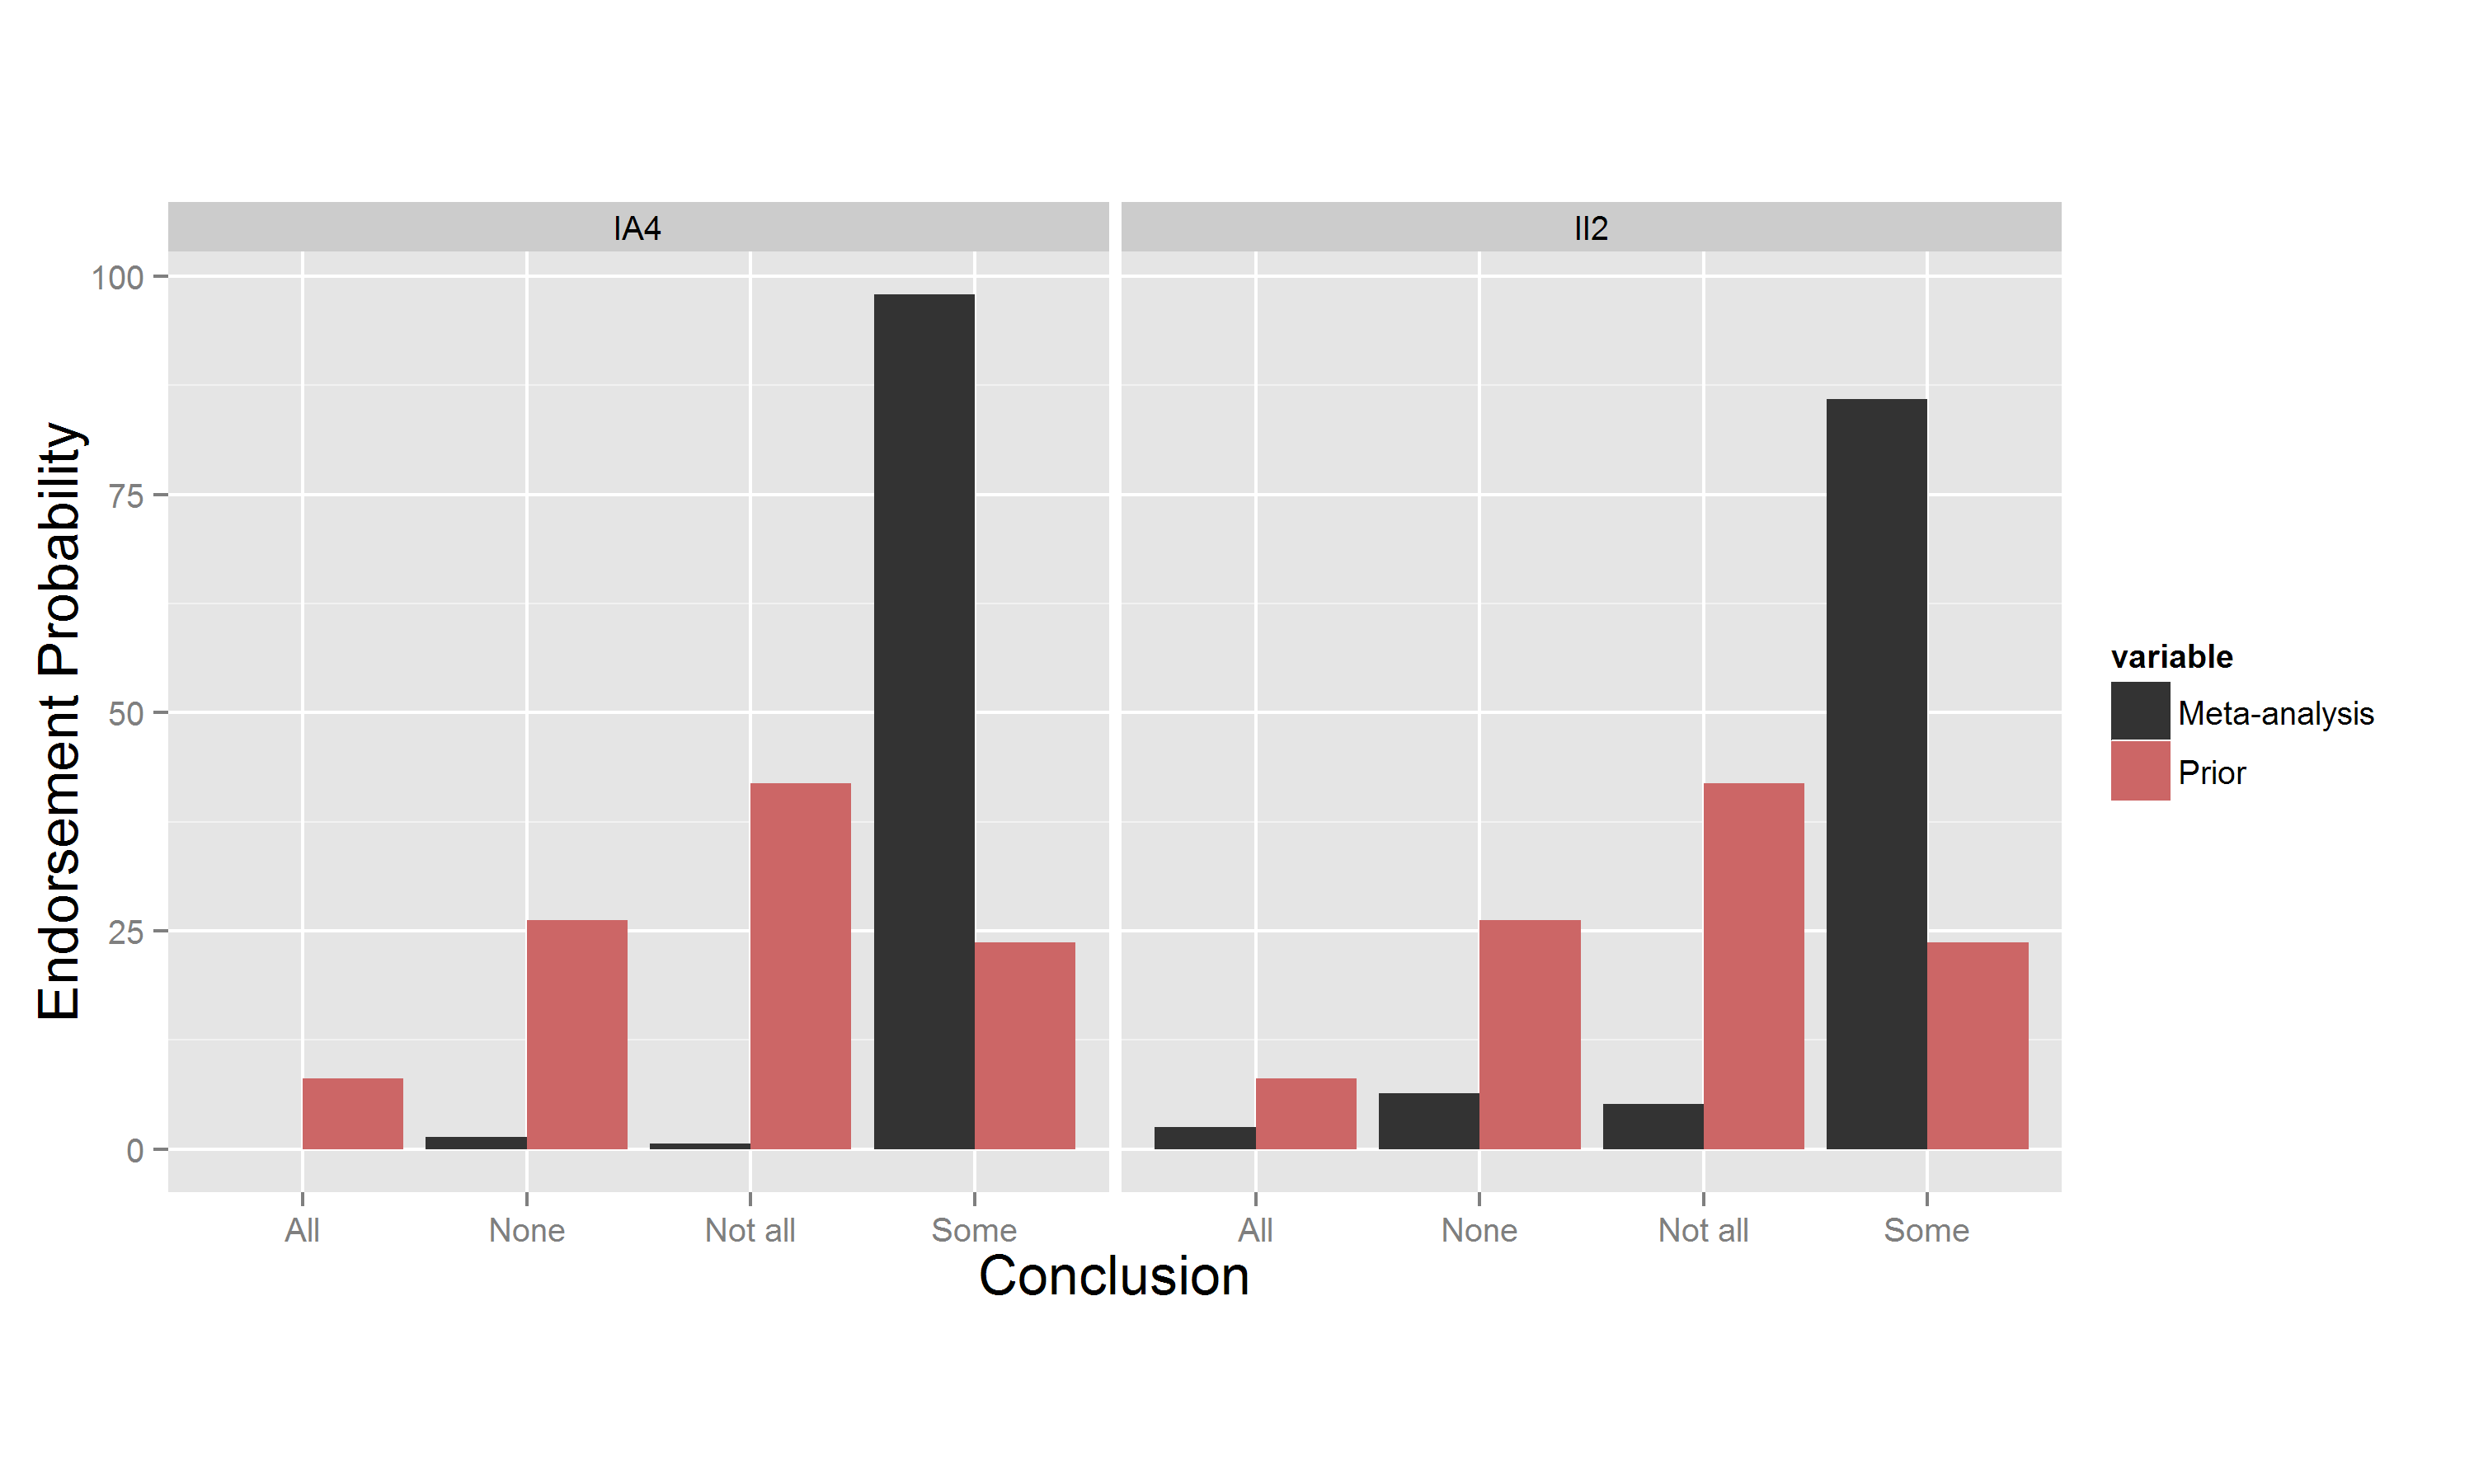
\includegraphics[width = {0.66\columnwidth}]{multibar_alpha1_prior}
%	\label{fig:subfigure1}}
%%\caption{Single-model, valid}}
%%\hfill
%\subfigure[conditional semantics]{ %}
%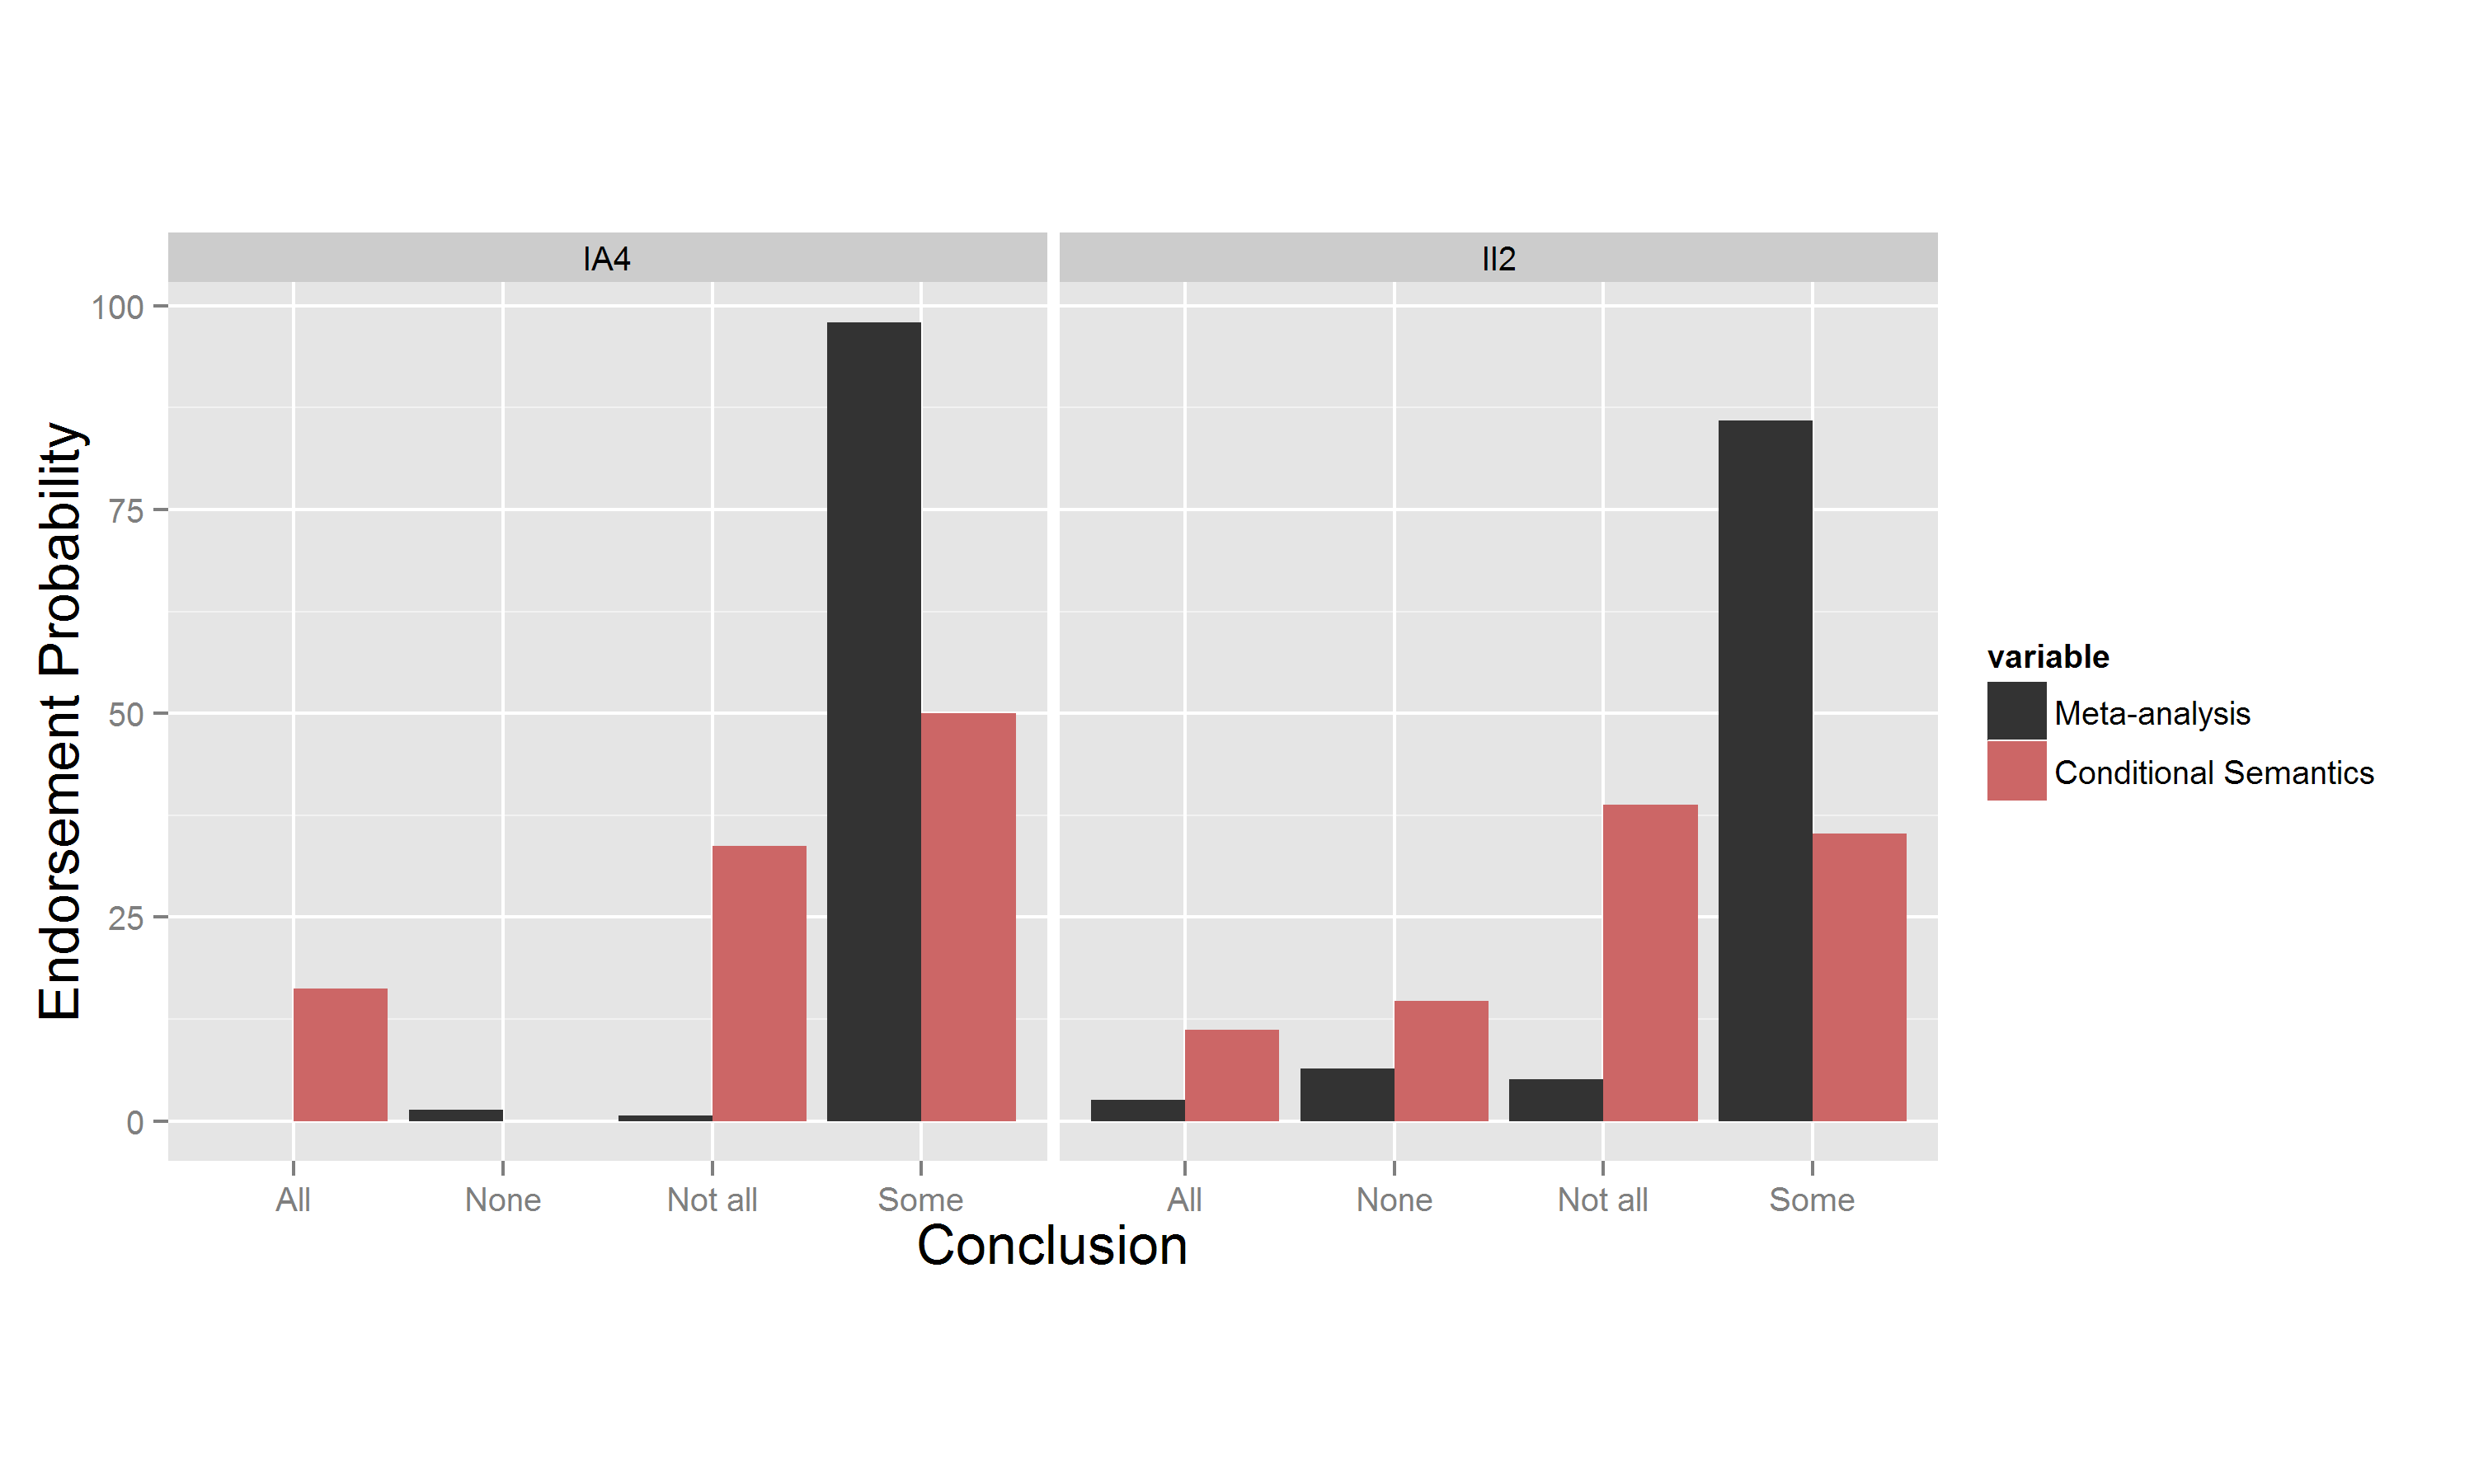
\includegraphics[width = {0.66\columnwidth}]{multibar_alpha1_lit}
%%\label{fig:subfigure3}
%\caption{Multiple-model, valid}
%}
%%\hfill
%\subfigure[conditional pragmatics]{
%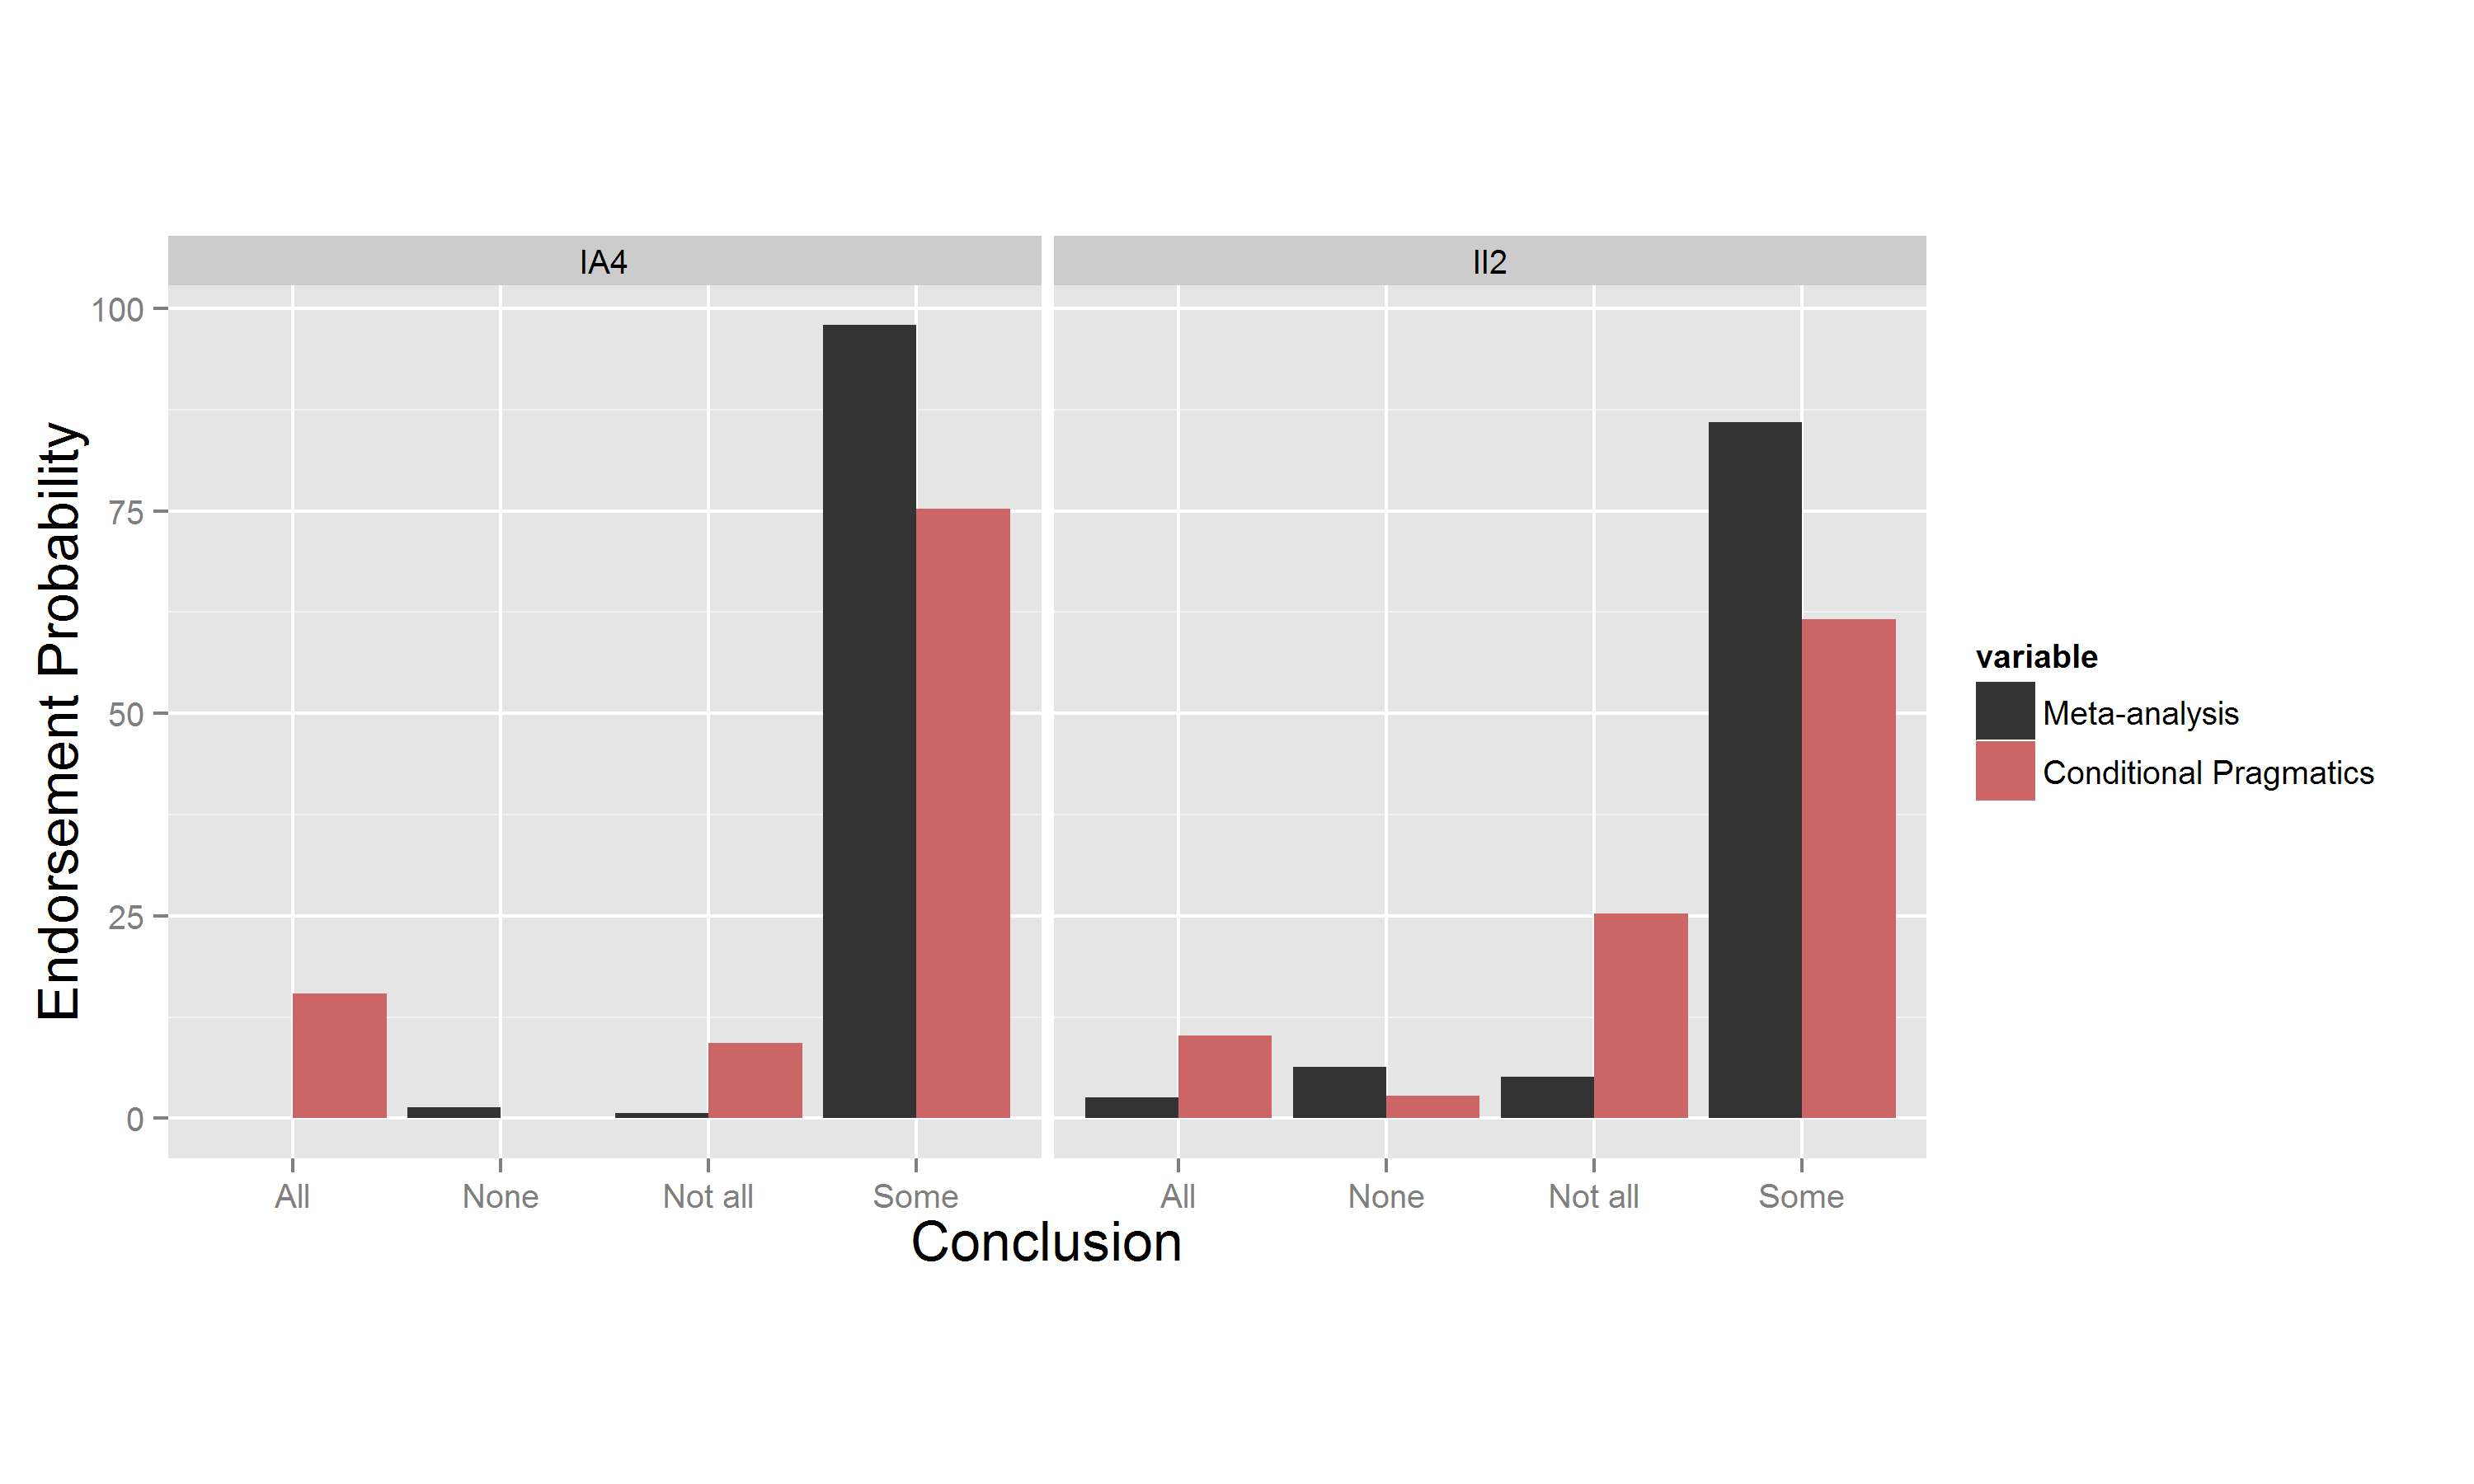
\includegraphics[width = {0.66\columnwidth}]{multibar_alpha1_prag}
%%\label{fig:subfigure5}
%\caption{invalid}
%%}
%%\quad
%%
%%\subfigure[one model, valid]{ %
%%\includegraphics[width = {0.66\columnwidth}]{IA4_boxplot_text}
%%%\label{fig:subfigure2}}
%%\hfill
%%\subfigure[multiple models, valid]{
%%\includegraphics[width = {0.66\columnwidth}]{EI3_boxplot_text}
%%%\label{fig:subfigure4}}
%%\caption{Multiple-model, valid}
%%\hfill
%%\subfigure[invalid]{
%%\includegraphics[width = {0.66\columnwidth}]{AA2_boxplot_text}
%%%\label{fig:subfigure6}}
%%\caption{invalid}
%%
%%\caption{Participants' endorsements in six syllogisms}
%%\label{fig:fig1}


%
%
%Mental Models Theory explains difficulty in syllogisms by demonstrating that multiple, distinct situations can be consistent with a pair of premises, giving rise to different possible conclusions. Valid syllogistic conclusions arise in every possible model. (This is the same notion of Pr(conclusion | premises) = 1). 
%
%This is always the case the logically invalid syllogisms (see discussion below), and is sometimes the case with logically valid syllogisms.

%\subsubsection{Logical invalidity}
%For syllogisms that have no valid conclusion, the probabilistic reasoner computes the probability of the conclusion conditioned on the premises being true by sampling. For all invalid syllogisms, this yield a gradeds response across the different possible conclusion types. 
%
%
%\subsubsection{Logical validity}
%A conclusion is logically valid if and if only it is true in all possible situations. Recall that possible situations are restricted to those that are consistent with the premises. The universal quantifiers (all, none) entail their particular counterparts (some, not-all), respectively. This was noticed by Aristotle and commonly visualized in the \emph{Square of Opposition}. For our probabilistic reasoner, confidence for {\emph all} and {\emph some} (to take the affirmative case) will be both maximal. {\emph All} is always true and {\emph some} is true whenever {\emph all} is true.


%We tested a number of rarity factors and found that p=0.25 provided the best fit. This is also consistent with the Probability Heuristic's rarity assumption. 


%\red{math here?}

%For reasoning over syllogisms, the prior distribution is conditioned on the truth of the premise sentences. This is the distribution over sentences conditioned on the fact that the premises are true. In this way, we evaluate the $\Pr$(conclusion $\arrowvert$ premises). This is essentially a metric of the plausibility of the argument. In this formulation, $\Pr$(conclusion $\arrowvert$ premises) = 1 if and only if the syllogism is logically valid.

%
%To set this parameter, we follow Johnson-Laird's principle of parsimony, which states that situations are constructed to ``maximize the number of properties of each individual to try to keep the number of \emph{distinct sorts} of individuals to a minimum".
%
%, from which we accept only those consistent with the premises \footnote{We follow J-L's lead by imposing the additionasl constraint that the syllogistic terms refer to non-empty classes in the world. This is the existential presupposition.}.
%
%The basic model has two parameters, which both contribute to the concept of Expected Value: situation size and property rarity. We tested a number of situation sizes and found 6 to be the best. This is consistent with Johnson-Laird's principle of parsimony which states that models are constructed to ``maximize the number of properties of each individual to try to keep the number of \emph{distinct sorts} of individuals to a minimum". 
%
%The number of distinct sorts of individuals is highest for logically invalid syllogisms precisely because the problems are not fully constrained. In Johnson-Laird's examples of these types of models, the number of individuals is always 6. 
%
%Rarity refers to the probability that a particular object in a world has a property (or belongs to class). A principle of rarity is often assumed in line with the intuition that properties are relative rare \footnote{This article is an article and it's about reasoning, but it's not a cat, and it's not a car, nor an elephant nor the color red. In fact, there's a very large number of things which this article is not.}, and we assume a principle of rarity here. We tested a number of rarity factors and found that p=0.25 provided the best fit. This is also consistent with Chater \& Oaksford's rarity assumption. 

%\subsection{Model predictions}






TODO after cogsci:
-implement phm (and mm?) for comparison.
-understand alpha param and pragmatic production recursion depth.
-understand the origin of symmetry breaking in 'prior' (i.e. funny prior which should be pragmatic).
-understand why pragmatic comprehender model doesn't work.
-analyze errors better.
-do experiments to get estimate of priors.
